\documentclass[12pt,a4paper,oneside]{book}
\usepackage[top=1in,bottom=1in]{geometry}
\usepackage{fontspec}
\usepackage{polyglossia}
\usepackage{hyperref}
\usepackage{titlesec}
\usepackage{tocloft}
\usepackage{fancyhdr}
\usepackage{tocloft}
\usepackage{setspace}
\usepackage{nonumonpart}
\usepackage{graphicx}
\usepackage{wrapfig}
\usepackage[usenames,dvipsnames]{color}
\setdefaultlanguage{malayalam}
\setmainfont[Script=Malayalam, HyphenChar="0000]{Rachana}
\lefthyphenmin=3
\righthyphenmin=4
\title{\fontsize{40pt}{1em}\selectfont \color{white}ലേഖനങ്ങളും കവിതകളും}
\author{\fontsize{20pt}{1em}\selectfont \color{white} പ്രൊഫ. സി വി ശങ്കരൻ}
\date{}
\newcommand{\sectionbreak}{\clearpage}
%= = = = = Formatting Hyperlinks in TOC = = = = =%
\hypersetup{
    colorlinks,
    citecolor=blue,
    filecolor=blue,
    linkcolor=blue,
    urlcolor=blue
}

%= = = = = Dots in TOC = = = = =%
\renewcommand{\cftchapleader}{\cftdotfill{\cftdotsep}}
\renewcommand{\cfttoctitlefont}{\hfil \Huge\vspace{1em}}

%= = = = = Formatting Chapter Style = = = = =%

\titleformat{\chapter}[hang]
  {\centering\LARGE}
  {\color{Gray}\thechapter}
  {10pt}
  {\\\centering\underline}
\titlespacing*{\chapter}{0cm}{0pt}{12pt}[0pt]

%= = = = = Multiple Parts in TOC = = = = =%
\makeatletter
\@addtoreset{chapter}{part}
\makeatother  

%= = = = = Formatting header and Footer = = = = =%
\pagestyle{fancy}
\renewcommand{\headrulewidth}{1pt}
\renewcommand{\footrulewidth}{1pt}
\usepackage{enumitem}
\usepackage{booktabs}
%= = = = = Document Begins = = = = =%
\begin{document}
\pagecolor{Maroon}
\maketitle
\pagenumbering{gobble}
\pagecolor{white}
\newpage
\renewcommand{\headrulewidth}{0pt}
\renewcommand{\footrulewidth}{0pt}
%------------------------------------------
\begin{table}[h!]

     \begin{tabular}{ c  p{.8\textwidth}}
     \raisebox{-.9\totalheight}{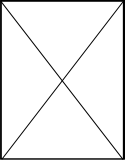
\includegraphics{image}}
      & 
      \parbox[t]{.8\textwidth}{\fontsize{25pt}{1em}{\selectfont സി വി ശങ്കരൻ}\\ 1956 ഡിസംബർ മാസത്തിൽ കോട്ടയം ജില്ലയിലെ കല്ലറ പെരുന്തുരുത്ത് കരയിൽ ചേലമറ്റത്തില്ലത്തു് ശ്രീ. വാസുദേവൻ ഇളയതിന്റേയും, ശ്രീമതി. സാവിത്രി അന്തർജനത്തിന്റേയും മൂന്നു് മക്കളിൽ രണ്ടാമനായി ജനിച്ചു. കല്ലറ മാണിക്യവിലാസം ഹയർ സെക്കൻഡറി സ്കൂളിലുമായി സ്കൂൾ വിദ്യാഭ്യാസം പൂർത്തിയാക്കി. കുറവിലങ്ങാട് എസ്‌ബി കോളേജിൽ നിന്നും രസതന്ത്രത്തിൽ ബിരുദവും, കോട്ടയം സിഎംഎസ് കോളേജിൽ നിന്ന് ബിരുദാനന്തരബിരുദവും കരസ്ഥമാക്കിയശേഷം പെരുമ്പാവൂർ വളയഞ്ചിറങ്ങര ശ്രീശങ്കര വിദ്യാപീഠം കോളേജിൽ രസതന്ത്ര വിഭാഗത്തിൽ അദ്ധ്യാപകനായി പ്രവേശിച്ചു. 2013 ജനുവരിയിൽ അവിടെനിന്നും പ്രൊഫസറായി വിരമിച്ചു.}
      
      \end{tabular}
      \end{table}
\noindent
ഭാര്യ : 

എൻ പ്രസന്നകുമാരി (റിട്ടയേഡ് പ്രൊഫസർ, ശ്രീ ശങ്കര കോളേജ്, കാലടി)\\
മക്കൾ : 

മനുശങ്കർ സി (അസി. പ്രൊഫസർ, ശ്രീ ശങ്കരവിദ്യാപീഠം കോളേജ്, വളയഞ്ചിറങ്ങര)

ബാലശങ്കർ സി (എംടെക് വിദ്യാർത്ഥി, ആദിശങ്കര എഞ്ചിനീയറിങ്ങ് കോളേജ്, കാലടി)
\noindent
മരുമക്കൾ ;

ശ്രീദേവി കേശവൻ (ബാങ്ക് ഓഫ് ഇന്ത്യ, കുറുപ്പും‌പടി, പെരുമ്പാവൂർ)
\\
\\
\textbf{\underline{വിലാസം}} : \\
ചേലമറ്റത്തില്ലം\\
മറ്റൂർ, കാലടി പി.ഓ\\
എറണാകുളം - 683574\\
ഈമെയിൽ : \href{mailto:cvsankaran@gmail.com}{cvsankaran@gmail.com}
           
             %------------------------------------------
\vfill
\noindent
ഈ പുസ്തകത്തിന്റെ ഡിജിറ്റൽ രൂപം \LaTeX എന്ന ടൈപ്‌സെറ്റിങ്ങ് സോഫ്റ്റ്‌വെയർ ഉപയോഗിച്ച് ഗ്നു/ലിനക്സ് ഓപ്പറേറ്റിങ്ങ് സിസ്റ്റത്തിൽ പ്രവർത്തിക്കുന്ന ഒരു കമ്പ്യൂട്ടറിൽ നിർമ്മിച്ചതാണ്. മലയാളം ലിപി ടൈപ്പ് ചെയ്യാനായി ഉപയോഗിച്ചിരിക്കുന്നത് രചന എന്ന ഫോണ്ടാണ്. ഈ പുസ്തകം ക്രിയേറ്റീവ് കോമൺസ് ബൈ ഷെയർ എലൈക് അനുമതിയിൽ പ്രസിദ്ധീകരിച്ചിരിക്കുന്നു.
\pagenumbering{gobble}
\hypersetup{
    colorlinks,
    citecolor=black,
    filecolor=black,
    linkcolor=black,
    urlcolor=black
}
\newpage
\tableofcontents
\newpage
\renewcommand{\headrulewidth}{1pt}
\renewcommand{\footrulewidth}{1pt}
\pagenumbering{arabic}
\onehalfspacing
%= = = = = Including Individual Chapters = = = = =%
%= = = = = Renaming ``Chapter'' = = = = =%
\makeatletter
\renewcommand{\@chapapp}{ലേഖനം}
\part{ലേഖനങ്ങൾ}

\setcounter{page}{1} %Start numbering pages
\chapter{അപ്പുവിന്റെ അത്ഭുതം}  
\obeylines
അപ്പു അഛനോടും അമ്മയോടുമൊപ്പം ഒരു വേളി കൂടാൻ നാട്ടിൽ പോയതാണു്. നേരത്തെ പോയാലേ എല്ലാവരുമായി വർത്തമാനം പറയാൻ പറ്റൂ എന്നു പറഞ്ഞു് അമ്മ ഉത്സാഹിച്ചതുകൊണ്ടു് നേരത്തെ അവിടെ എത്തിച്ചേർന്നു . അമ്മ, പറഞ്ഞതുപോലെ ഓരോരുത്തരോടും വർത്തമാനം പറഞ്ഞുകൊണ്ടു് നടന്നു. അഛൻ വേളിച്ചടങ്ങുകളിൽ സഹായിക്കാനും വിളമ്പാനും ക്രിയക്കു കൂടാനും ഒക്കെയായി പോയി. രണ്ടുപേരും അപ്പുവിനെ മറന്നതുപോലെ. അപ്പു ഒറ്റയ്ക്കായി. അപ്പു അലങ്കാരങ്ങളും ഒരുക്കങ്ങളും ഒക്കെ കണ്ട് അങ്ങനെ നില്കുകയായിരുന്നു.പെട്ടെന്നു പ്രായമായ ഒരു മുത്തശ്ശി വന്നു ചിരിച്ചു കൊണ്ടുചോദിച്ചു," എന്താ, ഉണ്ണി എന്നെ അറിയ്വോ ?. അപ്പുവിന്റെ മുത്തശ്ശി എന്റെ ഒരു ഏട്ടത്തിയാണു്" .അപ്പു വെളുക്കെ ചിരിച്ചു. മുത്തശ്ശിയും ചിരിച്ചിട്ടു പോയി. എന്തായാലും അപ്പുവിനു് മുത്തശ്ശിയെ ഇഷ്ടമായി. മുത്തശ്ശി പോയ വഴിയേ  നോക്കി നില്ക്കുകയായിരുന്നു അപ്പു.അപ്പുവിനേക്കാൾ പ്രായം കൂടിയ ഒരു കുട്ടി ഓടിവന്നു ചോദിച്ചു, " എന്താ അപ്പുക്കുട്ടൻ ഒറ്റയ്ക്കായിപ്പോയതു? എന്നെ അറിയുമോ? അപ്പുവിന്റെ അമ്മയും എന്റെ അമ്മയും ഒന്നിച്ചു പഠിച്ചവരാണു് ." അപ്പു ആ ചേച്ചിയെത്തന്നെ നോക്കിക്കൊണ്ടു മിണ്ടാതെ നിന്നു.
" അപ്പുക്കുട്ടാ തൊപ്പിക്കാരാ"  എന്നു പറഞ്ഞു ആ കുട്ടി ഓടിപ്പോയി.ആ കുട്ടിയുടെ ഓട്ടവും പാട്ടും കണ്ടു് അപ്പുവിനു് ചിരി വന്നു. അങ്ങനെ നില്ക്കുമ്പോളതാ രണ്ടുമൂന്നേട്ടന്മാർ വലിയ പത്രാസിൽ എന്തൊക്കെയോ പറഞ്ഞുകൊണ്ടു് വരുന്നു. അതിൽ, കണ്ണട വച്ചു മുടി ചപ്രശ്ശാ എന്നായ ഒരാൾ തന്നെ ചൂണ്ടി പറയുന്നതു് കേട്ടു. " ഇതു നമ്മുടെ കുഞ്ഞുണ്ണ്യേട്ടന്റെ പയ്യൻ അപ്പുവല്ലേ?." എന്നിട്ടു അപ്പുവിനോടായിപ്പറഞ്ഞു," തന്റെ മുത്തശ്ശന്റെ ഓപ്പോളുടെ മകളുടെ  മകനാണു് ഞാൻ" . ഇത്രയും പറഞ്ഞു് അവർ വിട്ടുപോയി. അപ്പുവിനു ഒരു പിടിയും കിട്ടിയില്ല. പിന്നെ ഓർത്തപ്പോഴാണു് രസം. ആ ഏട്ടന്റെ മുത്തശ്ശി തന്റെ മുത്തശ്ശന്റെ ഓപ്പോളാണു്. ചുരുക്കി പറയാവുന്ന കാര്യം എന്തിനിത്ര വളച്ചുകെട്ടിപ്പറയുന്നു? ഇതാണോ പത്രാസ്?
     അങ്ങനെ നില്ക്കുമ്പോൾ അഛനോടൊപ്പം സുമുഖനായ ഒരു ചെറുപ്പക്കാരനും തന്റെ പ്രായമുള്ള ഒരു കുട്ടിയും വന്നു. അഛൻ പറഞ്ഞു," കുഞ്ഞുകൃഷ്ണാ,ഇവനാണു് അപ്പു. അപ്പൂ, ഇതു് കൃഷ്ണൻ നായർ. മുത്തപ്ഫന്റെ മകളുടെ മകൻ. ഇതു് ഇയാളുടെ മകൻ സുരേഷ്. നിന്നെപ്പോലെ മൂന്നാം ക്ലാസ്സിൽ പഠിക്കുന്നു" . അപ്പോൾ " കുഞ്ഞുണ്ണീ, ഒന്നിങ്ങട് വരിക" എന്നു ആരോ വിളിയ്ക്കുന്നതു കേട്ടു അഛൻ പോയി. കൃഷ്ണൻ നായരും പോയി. ഉടൻ തന്നെ അമ്മയുടെ പ്രായമുള്ള ഒരു സ്ത്രീ കല്ല്യാണസ്സമ്മാനവും പ്ലാസ്റ്റിക് കൂട്ടിൽ തൂക്കി കടന്നു വന്നു." അപ്പുക്കുഞ്ഞല്ലേ,ഇതു? ഞാൻ ദേവകി വാരസ്യാർ. അപ്പുവിന്റെ അമ്മയുടെ ഇല്ലത്തിനടുത്താണു്" .ഒരിക്കൽ അമ്മാത്തു പോയപ്പോൾ ഇവരെ കണ്ടതു് അപ്പു ഓർത്തു. ഉടനെ അമ്മ എവിടെനിന്നോ ഓടിവന്നു. അപ്പുവിനെയും കൂട്ടി അച്ഛനെ തിരഞ്ഞു പിടിച്ചു. എന്നിട്ടു പറഞ്ഞു," നമുക്കു ഷാരടിമാഷിന്റെ വീടു വരെ ഒന്നു പോകണ്ടേ. മാഷ് വയ്യാതെ കിടക്കുകയാണല്ലോ. ഇനി എന്നാ ഇതിലേ വരാൻ പറ്റുകാ?"  
" ശരി, ആദ്യത്തെ പന്തി സദ്യ കഴിയുമ്പോഴേക്കും ഇങ്ങെത്തണം" എന്നു പറഞ്ഞു അഛൻ. എല്ലാവരും കൂടി കാറിൽ കയറിപ്പോയി.
    മാഷിന്റെ വീടിന്റെ പടിക്കൽ വണ്ടിയിട്ട് അകത്തേക്കു് നടക്കുമ്പോൾ ഒരു പൈക്കിടാവ് ഓടി വന്നു് അപ്പുവിന്റെ മുമ്പിൽ  കൂടി തുള്ളിച്ചാടിപ്പോയി. അപ്പുവിനു് വളരെ സന്തോഷമായി. നല്ല പൂങ്കുലയുള്ള ഒരു ചെടി കാറ്റിലാടി. പൂങ്കുല അപ്പുവിന്റെ തലയിൽ തൊട്ടുപോയി. ഒരു നായ ഓടിവന്നു് അഛന്റെ അരികിൽ വാലാട്ടിനിന്നു.ആകപ്പാടെ മുത്തശ്ശി പറഞ്ഞുതരാറുള്ള ശാകുന്തളത്തിലെ കണ്വാശ്രമം പോലെയുണ്ട്. അപ്പുവിനു പൈക്കുട്ടിയോടും പൂങ്കുലയോടും നായയോടും ഒക്കെ ഒരു മമതാബന്ധം തോന്നി.
   ഷാരടിമാഷ് മുൻ‌വശത്തുതന്നെ ഒരു ചാരുകസാലയിൽ കിടക്കുന്നുണ്ടായിരുന്നു. എല്ലവരേയും കണ്ടപ്പോൾ മാഷിനു് വളരെ സന്തോഷമായി.അപ്പുവിന്റെ തലയിൽ കൈവച്ച് അനുഗ്രഹിച്ചു. അപ്പുവിന്റെ അഛനേയും അമ്മയെയും അമ്മാവനേയും പഠിപ്പിച്ചിട്ടുള്ള മാഷാണു്. കുശലപ്രശ്നങ്ങൾക്കു ശേഷം കണ്വമഹർഷിയെക്കണ്ട പ്രതീതിയോടെ മടങ്ങിപ്പോന്നു.
       വേളിഹാളിൽ എത്തിയപ്പോഴേക്കും ആൾക്കാർ ഭൂരിഭാഗവും പോയിക്കഴിഞ്ഞിരുന്നു.ഒരു പന്തിയിൽ കുറച്ചുപേർ ഇരിക്കാൻ തുടങ്ങുന്നു. അവരുടെ കൂടെ കൂടി. ഒട്ടും തിരക്കില്ലാതെ സൗകര്യമായി സദ്യയുണ്ടു. ഇനിയും വർത്തമാനം പറയാൻ ആരുമില്ലാതിരുന്നതുകൊണ്ട് ഉടൻ തന്നെ എല്ലാവരും കാറിൽ കയറി തിരികെ പോന്നു. പോരുമ്പോൾ വഴിയിൽ എവിടെ നിന്നോ ഒഴുകിയെത്തിയ ഒരു ഗാനം കേട്ടു.
\hspace{2em}അറ്റമില്ലാത്തൊരീ ജീവിതപ്പാതയി-
\hspace{2em}ലൊറ്റയല്ലൊറ്റയല്ലൊറ്റയല്ലാ.
അപ്പു ഓർത്തുപോയി, അഛൻ, അമ്മ, മറ്റുബന്ധുക്കൾ, അവരുടെ ചാർച്ചക്കാർ, സുഹൃത്തുക്കൾ, പഠിപ്പിച്ച മാഷന്മാർ, എന്തിനധികം? തൊടിയിലെ ചെടികൾ, വളർത്തുന്ന ജീവികൾ, ഇവയോടെല്ലാം ഒരു അടുപ്പം തോന്നുന്നു.
അപ്പു അത്ഭുതത്തോടെ അറിയാതെ ചോദിച്ചുപോയി" നമ്മൾക്ക് ഒരുപാട് ആൾക്കാരുണ്ട്. അല്ലേ അഛാ?." 
അതെന്താ അപ്പൂ, അങ്ങനെ ചോദിച്ചത്?." 
എത്ര ആളുകളാ എന്നെ ശ്രദ്ധിക്കുകയും കുശലം പറയുകയും ചെയ്യുന്നത്! മാഷിന്റെ വീട്ടിലെ പൈക്കിടാവും നായയും ചെടികളും പോലും എന്നെ ശ്രദ്ധിച്ചതുപോലെ തോന്നി.
അഛൻ പറഞ്ഞു,, " ഈ പ്രപഞ്ചത്തിലെ എല്ല സൃഷ്ടിജാലങ്ങളും ഒരേ ഈശ്വരന്റെ ചൈതന്യം ഉൾക്കൊള്ളുന്നു. എല്ലാ ജീവജാലങ്ങളും ഒരേകുടുംബത്തിലെ അംഗങ്ങളാണു് .മഹാകവി വള്ളത്തോൾ പാടിയിട്ടില്ലേ,
\begin{center}
" ലോകമേതറവാടു തനിയ്ക്കീചെടികളും പുൽക്കളും പുഴുക്കളും കൂടിത്തൻ കുടുംബക്കാർ" .
\end{center}

\chapter{ഏട്ടാ....ഏട്ടാ...അനിയാ...അനിയാ..}
\obeylines
കർക്കടകത്തിലെ ഒരു ഞായറാഴ്ച. കുട്ടികളുമായി അമ്പലത്തിൽ പോയി തൊഴീൽ കഴിഞ്ഞു മതില്ക്കു പുറത്തിറങ്ങി. ആനപ്പന്തലിൽ ഏട്ടനും അനിയനും ഓട്ടം തന്നെ ഓട്ടം. സ്ക്കൂളില്ലാത്തതും ഓടിക്കളിയ്ക്കാൻ സ്ഥലം കിട്ടിയതും ആഘോഷിയ്ക്കുകയാണവർ. കുറേ ഓടിത്തളർന്നപ്പോൾ തിരികെപ്പോകുവാൻ സമ്മതിച്ചു. എല്ലാവരും കൂടി വീടെത്തി. എത്തിയ ഉടനെ രണ്ടുപേരും ധാരാളം വെള്ളം കുടിച്ചു. ഉടനെതന്നെ ജ്യേഷ്ഠൻ പോക്കറ്റിൽനിന്നും ഒരു പടം എടുത്തുപൊക്കിപ്പിടിച്ചു. അമ്പലത്തിൽ വെച്ചു എപ്പോഴോ സ്വാമിസ്സാർ കൊടുത്ത ശ്രീരാമന്റെ പടം. പടം കണ്ടപ്പോൾ അനിയന്‌ അതു കിട്ടണമെന്നായി. ഏട്ടനായ അപ്പു കൊടുത്തില്ല.അനിയൻ പിടിച്ചുവാങ്ങാൻ ശ്രമിച്ചു. ഏട്ടൻ അതും കൊണ്ടോടി. അനിയൻ പുറകെ ഓടി. രണ്ടുപേരും വീണ്ടും ഓട്ടം തന്നെ.
“അപ്വേ, നീ അന്യേനെ ഇങ്ങനെ ഓടിയ്ക്കാതെ” അമ്മ വിളിച്ചുപറഞ്ഞു.
അവരുണ്ടോ ഓട്ടം നിറുത്തുന്നു. ഇനി എന്താചെയ്ക? അമ്മ അവിടെയൊക്കെ നോക്കി. ഒരു ശ്രീകൃഷ്ണന്റെ പടം കിട്ടി. അതു അനിയന്റെ നേരേ നീട്ടി. അയാൾക്കതു പോരാ. ഏട്ടന്റെ കൈവശം ഉള്ള പടം തന്നെ വേണം. ഏട്ടൻ കൊടുക്കുകയുമില്ല. അനിയനു വേണം താനും. കുട്ടികൾക്കു വാശി കൂടിവന്നു. കുട്ട്യോൾടെ അച്ഛൻ എത്തിയിട്ടില്ല. ഇനി എന്താ വേണ്ടേ എന്നുവിചാരിച്ചു നില്ക്കുമ്പോൾ അതാ വാസ്വഫൻ പടികടന്നു വരുന്നു. ആശ്വാസമായി.
“കുട്ടികളേ,ആരാ വരുന്നതെന്നു നോക്കിയ്ക്കേ” അമ്മ വിളിച്ചുപറഞ്ഞു.
“വാസ്വഫൻ” രണ്ടുപേരും ഒരുമിച്ചു വിളിച്ചുപറഞ്ഞു.
വാസ്വഫനെ രണ്ടുപേർക്കും ഇഷ്ടമാണ്‌. വല്ല്യ വല്ല്യ കാര്യങ്ങൾ അഛനോടു സംസാരിയ്ക്കും. പലഹാരത്തിന്റെ കാര്യങ്ങൾ അമ്മയോടു സംസാരിയ്ക്കും. കുട്ടികൾക്കു കപ്പലണ്ടി കൊടുക്കും, കഥകൾ പറഞ്ഞുതരും. രണ്ടുപേരും തത്ക്കാലം വാശിയെ കാശിയ്ക്കു വിട്ടിട്ട് വാസ്വഫനടുത്തേയ്ക്കെത്തി.
“എന്താ അപ്പ്വേ കയ്യിലെ ചിത്രം? ശ്രീരാമനാ?ആയ്! രാമായണമാസം അല്ലേ? പണ്ടൊക്കെ ഇടവം മിഥുനം കർക്കടകം ചിങ്ങം എന്നൊക്കെയാ പറയാറ്‌. ഇപ്പോൾ അങ്ങനെയല്ല. കർക്കടകം ഇല്ല. പകരം രാമായണമാസം എന്നാപറയുക. മിഥുനത്തിലെ പെരുമഴയ്ക്കുശേഷം വരുന്ന കള്ളക്കർക്കടകം ഒരു പഞ്ഞമാസം തന്നെ. എത്ര ധനവാനും ഒരു ഇടിച്ചിൽ ഉണ്ടാവും. ഒന്നും നട്ടാൽ മുളയ്ക്കാത്ത, ഒന്നും ചെയ്യാൻ പറ്റാത്ത കാലം.
“കർക്കടമാസം കഴിയും വരേയ്ക്കിനി-
ക്കഞ്ഞിയാണുണ്ണി നിനക്കിഷ്ടമാവുമോ?”
എന്നാണ്‌ ഉണ്ണിയോട് അമ്മ ചോദിക്കുന്നത്. ഏതായാലും ഇപ്പോൾ മറ്റൊന്നുമില്ലെങ്കിലും കർക്കടകമാസതിൽ രാമായണം വായന നടക്കുന്നുണ്ട്. അതുകൊണ്ടാവാം ഇപ്പോൾ ദാരിദ്ര്യവും അല്പം കുറവുണ്ട്”.
അപ്പോഴേയ്ക്കും അമ്മ സംഭാരവുമായി വന്നു.അഫൻ സംഭാരം കുടിച്ചുകഴിഞ്ഞപ്പോൾ “ഇനി കഥ, ഇനി കഥ” എന്നുപറഞ്ഞു കുട്ടികൾ തിടുക്കം കൂട്ടി.
“കഥ മാത്രമല്ല കപ്പലണ്ടിയുമാവാം. നിങ്ങളുടെ ഓട്ടവും ബഹളവും കണ്ട് അതിന്റെ കാര്യം വിട്ടുപോയി”. ഓരോപൊതി കപ്പലണ്ടി രണ്ടു പേർക്കും കൊടുത്തു. എന്നിട്ട് പറഞ്ഞുതുടങ്ങി
“എന്നും രാമായണം വായിയ്ക്കുന്നുണ്ടല്ലോ. അതു ഭാഷാസ്വാധീനം ഉണ്ടാക്കും. ഇന്ന് നമുക്ക് രാമായണത്തിലെ ചിലരെ പരിചയപ്പെടാം. ആദ്യമേതന്നെ നിങ്ങളെപ്പോലെ ഓടിക്കളിയ്ക്കുന്ന, അല്ല, പറന്നു കളിയ്ക്കുന്ന ഒരേട്ടനും അനിയനും ആവട്ടെ. ഗരുഡൻ എന്നു കേട്ടിട്ടില്ലെ?”
“ഉവ്വ്, മഹാവിഷ്ണുവിന്റെ വാഹനം” - അപ്പു.
“ഗരുഡന്‌ ഒരേട്ടൻ ഉണ്ട്.അരുണൻ.”
“അരുണൻ എന്നൽ “അര”ണൻ എന്നല്ലെ?” - വീണ്ടും അപ്പു.
“അതെയതെ. അരയ്ക്കു കീഴ്ഭാഗം ഇല്ലാത്തയാൾ. സൂര്യരഥത്തിന്റെ തേരാളി.”
“സൂര്യന്റെ തേരിന്‌ ഏഴു കുതിരകളാണ്‌. അല്ലേ?”
“എന്നുപറഞ്ഞാൽ ഏഴു നിറങ്ങൾ ചേർന്നാണ് സൂര്യരശ്മിയുണ്ടായിരിയ്ക്കുന്നത് എന്നാണർത്ഥം”.
“മാനത്തെ മഴവില്ലിനേഴുനിറം
മനസ്സിന്റെ മാരി വില്ലിനേഴല്ലെഴുനൂറ്‌” അപ്പു ഒരു പാട്ടു പാടി
“മഴവില്ലിനും ഏഴു നിറമല്ല. എത്രയെന്നു പറയാൻ പറ്റുകയില്ല. അതൊക്കെ പ്രകാശത്തിന്റെ സ്വഭാവത്തെപ്പറ്റി കൂടുതൽ പഠിയ്ക്കുമ്പോൾ മനസ്സിലാകും. ഏതായാലും സൂര്യന്റെ ഡ്രൈവറായ അരുണൻ വിവാഹം കഴിച്ചു. ശ്യേനി അഥവാ മഹാശ്വേത”.
“അരുണം ചുവപ്പും ശ്വേതം വെളുപ്പും” കഴിഞ്ഞ ദിവസം ക്ലാസ്സിൽ രക്തത്തെപ്പറ്റി പഠിച്ചതോർത്ത് അപ്പു പറഞ്ഞു.
അഫൻ തുടർന്നു “അരുണനും ശ്യേനിക്കും രണ്ടു മക്കൾ. രണ്ടു കഴുകന്മാർ. ഏട്ടന്റെ പേര്‌ സമ്പാതി. അനുജൻ ജടായുസ്സ് അഥവാ ജടായു.
\begin{center}
അരുണപ്രിയയാം ശ്യേനി
പെറ്റൂ രണ്ടു കുമാരരെ
സമ്പാതിയെന്നു വൻപേറും
ജടായുസ്സെന്നുമങ്ങനെ
\end{center}
കുട്ടിക്കാലത്തു ഇവർ ഒന്നു പറന്നു കളിച്ചു. ആർക്കാണു കൂടുതൽ ഉയരത്തിൽ പറക്കാൻ കഴിയുന്നതെന്നറിയാൻ വാശിയോടെ മേല്പ്പോട്ടു പറന്നുയർന്നു. കൂടുതൽ ഉയരത്തിലേയ്ക്കു പോയ അനുജൻ ജടായുവിനു സൂര്യന്റെ ചൂടേറ്റ് ഒരു തളർച്ച അനുഭവപ്പെട്ടു. ഉടൻ തന്നെ ഏട്ടനായ സമ്പാതി ജടായുവിനു മുകളിൽ ഉയർന്നുപൊങ്ങി ചിറകു വിരിച്ചു പറന്നുനിന്നു തണലേകി. പക്ഷേ, എന്തു സംഭവിച്ചു? സൂര്യന്റെ ചൂടേറ്റു സമ്പാതിയുടെ ചിറകുകൾ കരിഞ്ഞുപോയി. സമ്പാതി താഴേക്കു വീണു, വിന്ധ്യപർവതത്തിൽ നിശാകരമുനിയുടെ ആശ്രമത്തിൽ. ശിഷ്ടകാലം മുനി ആഹാരം നല്കി സമ്പാതിയെ രക്ഷിച്ചു. സമ്പാതിയും ജടായുവും സീതാന്വേഷണത്തിൽ ശ്രീരാമനു സഹായികളായ കഥകൾ രാമായണത്തിൽ പറയുന്നുണ്ട്.
“ഓടിക്കളിക്കുമ്പോൾ അനിയൻ വീഴാതെ നോക്കേണ്ടതു ഏട്ടനാണെന്നാണ്‌ അഫൻ പറഞ്ഞുവരുന്നത്, കേട്ടോ അപ്പൂ” കഥ കേട്ടുകൊണ്ടു വന്ന അഛൻ പറഞ്ഞു.
“ഏട്ടൻ അനിയനെ രക്ഷിക്കുന്ന കാര്യമേ ഉള്ളൂ? അനിയനു എന്തും ആകാം,അല്ലേ?”അപ്പു പരിഭവിച്ചു
വാസ്വഫൻ തുടർന്നു
“രാമായണത്തിൽ തന്നെയുണ്ടല്ലോ നാലു ജ്യേഷ്ഠാനുജന്മാർ. നീണ്ട പതിന്നാലു വർഷം കൊടുങ്കാട്ടിലും മലയിലുമായി രാക്ഷസന്മാരുടെയും വന്യമൃഗങ്ങളുടെയുമിടയിൽ രാമേട്ടന്റെ സഹായിയായി ഒരനുജൻ ലക്ഷ്മണൻ. സ്വന്തം അമ്മയെയും ഭാര്യയേയും കൊട്ടാരത്തിൽ വിട്ട് തനിക്കുവേണ്ടിയല്ല, ഏട്ടനു വേണ്ടി ഇത്ര കഷ്ടപ്പാടുകൾ സഹിച്ചു ജീവിച്ച മറ്റൊരനുജൻ പുരാണത്തിലെങ്ങുമില്ല”.
“സമ്പാതി എന്ന ഏട്ടൻ അനിയനെ രക്ഷിച്ചതിലും എത്രയധികമാണ്‌ ലക്ഷ്മണൻ എന്ന അനുജൻ ചെയ്തിരിക്കുന്നത്. കൂയ്! കൂയ്! അനിയനാണ്‌ കൂടുതൽ മഹാൻ” അനിയൻ തുള്ളിച്ചാടി.
“കഥ തീർന്നില്ലല്ലോ” വാസ്വഫൻ ഇടപെട്ടു “തനിയ്ക്കവകാശപ്പെട്ട രാജപദവിയും കൊട്ടാരങ്ങളും ഭരതനു വേണ്ടി ഉപേക്ഷിച്ചിട്ടാണല്ലൊ ശ്രീരാമൻ കാട്ടിലേയ്ക്കു പോയത്”
“ഇപ്പോഴോ” അപ്പുവിനു കുറച്ചുകൂടി ഗമയായി.
“അതു വേറെ അനിയനല്ലേ” അനിയനും വിട്ടുകൊടുക്കാൻ തയ്യാറല്ല.
വാസ്വഫൻ ഇടപെട്ടു, “അവർ നാലു ജ്യേഷ്ഠാനുജന്മാരും പരസ്പരം സ്നേഹിച്ചും ബഹുമാനിച്ചുമാണ്‌ കഴിഞ്ഞിരുന്നത്. അത് രാമായണം കഥ മുഴുവൻ വായിച്ചാൽ മനസ്സിലാകും. അരും ആരെയുംകാൾ കേമനല്ല. ഇനിയുമുണ്ട് അനവധി ഏട്ടന്മാരും അനവധി അനിയന്മാരും
രാമാദികൾ നാലു സഹോദരന്മാരെപ്പോലെ രാവണാദികൾ നാലു സഹോദരങ്ങൾ. വൈശ്രവണൻ, രാവണൻ, കുംഭകർണൻ, വിഭീഷണൻ. ഇവരെല്ലാവരും വിശ്രവസ്സ് എന്ന മഹർഷിയുടെ പുത്രന്മാരാണ്‌. ഇവരിൽ വൈശ്രവണൻ യക്ഷന്മാരുടെ രാജാവും രാവണൻ രാക്ഷസന്മാരുടെ രാജാവും. തെക്കേ സമുദ്രത്തിൽ ത്രികൂടപർവതത്തിനു മുകളിൽ ഇന്ദ്രന്റെ രാജധാനിയെ വെല്ലുന്ന ഒരു നഗരം വിശ്വകർമാവു രാക്ഷസന്മാർക്കുവേണ്ടി ഉണ്ടാക്കിക്കൊടുത്തിരുന്നു. അവർ മഹാവിഷ്ണുവിനോടുണ്ടായ യുദ്ധത്തിൽ പരാജിതരായി പാതാളത്തിൽ പോയി ഒളിച്ചു പാർത്തു വരികയായിരുന്നു. അങ്ങനെ ശൂന്യമായിക്കിടന്ന ലങ്കയിൽ വിശ്രവസ്സിന്റെ നിർദ്ദേശപ്രകാരം വൈശ്രവണനെന്ന കുബേരൻ താമസമാക്കി. ലങ്കയെ സംരക്ഷിച്ചു ഐശ്വര്യം നിലനിർത്തി. സമുദ്രത്തിനു നടുവിലുള്ളദ്വീപിൽ നിന്നു പുറത്തേയ്ക്ക് പോകാൻ കുബേരനു മൂന്നു വിമാനങ്ങൾ ഉണ്ടായിരുന്നു. അതിൽ ഏറ്റവും കേമം ഭൂമിയിൽ ഒരിടത്തു നിന്നു മറ്റൊരിടത്തേക്ക്പോകുവാൻ ഉപയോഗിച്ചിരുന്ന പുഷ്പകവിമാനമാണ്‌. മറ്റു വിമാനങ്ങൾ ഭൂമിയിൽനിന്നു പുറത്തേക്കു പോകുവാനുള്ളതാണ്‌.
ഇങ്ങനെയിരിയ്ക്കുന്ന കാലത്താണ്‌ വിശ്രവസ്സിനു മറ്റു മൂന്നുപുത്രന്മാരുണ്ടാകുന്നത്. അവർ ബ്രഹ്മദേവനെ തപസ്സു ചെയ്ത് വലിയ വരങ്ങളൊക്കെ സമ്പാദിച്ചു തിരിച്ചു വന്നപ്പോൾ അവരുടെ അമ്മാത്തുമുത്തശ്ശനായ സുമാലിയും കൂട്ടരും രാവണനെ രാക്ഷസവംശത്തിന്റെ അധിപനായി അവരോധിച്ചു സ്വീകരിയ്ക്കുകയും രാക്ഷസന്മാർക്കവകാശപ്പെട്ട ലങ്ക കുബേരനിൽനിന്നു തിരിച്ചുപിടിയ്ക്കാൻ ആവശ്യപ്പെടുകയും ചെയ്തു. എന്നാൽ ജ്യേഷ്ഠനോട് അവിടെനിന്നു ഇറങ്ങിപ്പോകാൻ പറയാനുള്ള മടി കൊണ്ടങ്ങനെ പറഞ്ഞില്ല. വീണ്ടും സുമാലിയുടെയും കൂട്ടരുടെയും നിർബ്ബന്ധം കൂടിവന്നപ്പോൾ രാക്ഷസന്മാർക്കവകാശപ്പെട്ട ലങ്ക അവർക്കു തിരികെ നല്കണമെന്നു വളരെ മാന്യമായി ആവശ്യപ്പെട്ടു. ഏട്ടനായ വൈശ്രവണനാകട്ടെ അഛന്റെ അഭിപ്രായവും നിർദ്ദേശവും അനുസരിച്ച് ലങ്ക അനിയനും കൂട്ടർക്കും ഒഴിഞ്ഞു കൊടുത്ത് അളകാപുരിയിലേയ്ക്കുപോയി. എത്ര ഭംഗിയായിട്ടാണു ജ്യേഷ്ഠാനുജന്മാർ പെരുമാറിയത് പിന്നീടങ്ങോട്ടു രാവണന്റെ സ്വഭാവം ആകെപ്പാടെ മാറിപ്പോയി.”
“ഇനിയുമില്ലെ, അഫാ, മറ്റൊരേട്ടനും അനിയനും? ഞങ്ങൾ അടികൂടുമ്പോൾ മുത്തശ്ശൻ പറയാറുണ്ട് ‘ബാലിസുഗ്രീവന്മാർ’ തുടങ്ങി എന്ന്” - അപ്പു
“ശരിയാണ് പരസ്പരസ്നേഹത്തിന്റെയും ബഹുമാനത്തിന്റെയും ഉദാഹരണമായിരുന്നു ബാലി സുഗ്രീവന്മാർ.”
“അതു രണ്ടു കുരങ്ങന്മാരല്ലേ? അപ്പോ അടികൂടും”അനുജൻ
“അല്ല അവർ ജന്മനാ കുരങ്ങന്മാരല്ല. ജടായുവിന്റെയും സമ്പാതിയുടെയും അഛനായ അരുണൻ ഇവരുടെ അമ്മയാണ്‌ ഒരു ദിവസം അസ്തമയത്തിനുശേഷം അരുണൻ സൂര്യരഥം ഷെഡ്ഡിൽ കയറ്റിയിട്ട് സ്ത്രീരൂപം ധരിച്ചു ഇന്ദ്രസഭയിൽ അപ്സരസ്സുകളുടെ നൃത്തം കാണാൻ പോയി. പുതിയ കാഴ്ചക്കാരിയെ ഇന്ദ്രനു വളരെയധികം ഇഷ്ടപ്പെട്ടതുകൊണ്ട് അവൾക്ക് ഇന്ദ്രനിൽനിന്നും ഒരു കുട്ടിയെ ലഭിച്ചു. ഇക്കാരണത്താൽ അരുണൻ തേരിലെത്താൻ താമസിച്ചു. സൂര്യന്റെ പ്രയാണം വൈകി. അരുണനോട് സൂര്യൻ ദേഷ്യപ്പെട്ടു. കാരണം അറിഞ്ഞപ്പോൾ ആദിത്യനും ആ സ്ത്രീരൂപം ഒന്നുകാണണമെന്നുതോന്നി. അതു സാധിച്ചുകൊടുത്തപ്പോൾ സൂര്യനിൽനിന്നും ഒരു കുട്ടിയെ ലഭിച്ചു. അങ്ങനെ അരുണനു, അല്ല, അരുണിയ്ക്ക്, രണ്ടു കുട്ടികളായി.”
“മഹാവിഷ്ണുവിന്റെ മോഹിനീരൂപത്തിൽക്കൂടി ശിവന്റെ പുത്രനായി ശാസ്താവ് ജനിച്ചതുപോലെ, അല്ലേ?” അപ്പു.
“അതെ, രണ്ടു കുട്ടികളെയും ഇന്ദ്രന്റെ നിർദ്ദേശപ്രകരം വളർത്തുവാനായി അഹല്യയെ ഏല്പ്പിച്ചു. ഒരു ദിവസം കുട്ടികളെ പുഴയിൽ കൊണ്ടു പോയി കുളിപ്പിച്ച് അഹല്യ രണ്ടെളിയിലുമായി എടുത്തുകൊണ്ടുവരുന്നതു കണ്ട് മഹർഷി ഗൗതമനു കോപം വന്നു. കോപം വന്നാൽ എന്താചെയ്ക? ശപിച്ചു. കുരങ്ങുകുട്ടികൾ തള്ളക്കുരങ്ങിനെ അള്ളിപ്പിടിചുകൊണ്ടുവരുന്നതുപോലെ കണ്ടിട്ടു കുട്ടികൾക്കു കുരങ്ങിന്റെ സ്വഭാവം ആകട്ടെ എന്നാണ്‌ ശപിച്ചത്. അന്നുമുതൽ അവർ മർക്കടന്മാരായി. ഇതറിഞ്ഞു ദേവേന്ദ്രൻ രണ്ടു കുട്ടികളെയും കൊണ്ടുപോയി നന്ദനവനത്തിൽ താമസിപ്പിച്ചു. അക്കാലത്തു കിഷ്കിന്ധ എന്ന രാജ്യം വാണിരുന്ന മർക്കടരാജാവായ ഋക്ഷരജസ്സ് കുട്ടികളില്ലാതെ ദു:ഖിച്ചിരുന്നു. മന്ത്രിയായ ജാംബവാന്റെ നിർദേശപ്രകാരം ദേവേന്ദ്രനോടു പ്രാർത്ഥിച്ചതനുസരിച്ച് ഈ രണ്ടു കുട്ടികളെയും ഋക്ഷരജസ്സിനു നല്കി. വാലിനു ഭംഗിയുള്ളതുകൊണ്ട് ഇന്ദ്രപുത്രനു ബാലി എന്നും കഴുത്തിന്റെ ഭംഗി കണ്ടു സൂര്യപുത്രനു സുഗ്രീവൻ എന്നും പേരു നല്കിയിരുന്നു. ഋക്ഷരജസ്സിന്റെ കാലശേഷം മൂത്തവനായ ബാലി ചക്രവർത്തിയായും സുഗ്രീവൻ ഇളയരാജാവായും മന്ത്രിമാരോടുകൂടി വാണരുളുകയായിരുന്നു. അപ്പോഴാണ്‌ മായാവി എന്ന അസുരനുമായി ബാലിയ്ക്കു യുദ്ധം ചെയ്യേണ്ടി വന്നത്. യുദ്ധം ചെയ്തു ചെയ്തു രണ്ടുപേരും ഒരു ഗുഹയിൽക്കയറി. രക്തം കാണുകയാണെങ്കിൽ ഗുഹയടച്ചുപൊയ്ക്കൊൾവാൻ ബാലി സുഗ്രീവനു നിർദ്ദേശം നല്കി. ഒരുവർഷം കാത്തുനിന്നിട്ടും ആരും പുറത്തു വന്നില്ല. പക്ഷേ രക്തത്തിന്റെ പ്രളയം വന്നപ്പോൾ സുഗ്രീവൻ ഗുഹയടച്ചുപോയി കിഷ്ക്കിന്ധയിലെ രാജാവായി. പക്ഷേ മരിച്ചതു മായാവിയായിരുന്നു. ബാലി പുറത്തിറങ്ങാൻ വന്നപ്പോൾ ഗുഹയടച്ചിരിയ്ക്കുന്നതുകണ്ടു ദേഷ്യത്തോടെ തള്ളിത്തുറന്നു സുഗ്രീവനുമായി വഴക്കിട്ടു രാജ്യം കൈക്കലാക്കി. അന്നു രാജാവായിരുന്ന സുഗ്രീവനു വേണമെങ്കിൽ ബാലിയെ വധിയ്ക്കാമായിരുന്നു. പക്ഷേ, ജ്യേഷ്ഠനായതുകൊണ്ടു സുഗ്രീവൻ അതു ചെയ്തില്ല. സുഗ്രീവൻ എന്തൊക്കെപ്പറഞ്ഞിട്ടും ബാലിയ്ക്കു വിശ്വാസമായില്ല. ബാലി പുറത്തിറങ്ങാതിരിയ്ക്കാൻ വേണ്ടിത്തന്നെയാണ്‌ഗുഹയടച്ചതെന്നു വിശ്വസിച്ചു. ആ വൈരം പിന്നീട് തുടരുകയും ചെയ്തു. പരസ്പരസ്നേഹത്തോടുകൂടി പെരുമാറിയിരുന്ന അവർക്കിടയിൽ ഉണ്ടായ തെറ്റിദ്ധാരണയാണ് അകൽച്ചയ്ക്കു കാരണമായത്.
ഇങ്ങനെ നോക്കിയാൽ അടിസ്ഥാനപരവും സുദൃഢവും ആയ സഹോദരസ്നേഹത്തെ വിശദമാക്കുന്നതാണ് രാമായണത്തിലെ പല കഥാഭാഗങ്ങളും. മഹാഭാരതത്തിലാണെങ്കിൽ രണ്ടു തായ്‌വഴികളിലെ സഹോദരന്മാർ തമ്മിൽ സ്വത്തിനു വേണ്ടി നടത്തുന്ന വഴക്കുകളാണ്. രാമായണസഹോദരന്മാർ തമ്മിൽ സ്വത്തു തർക്കം ഉണ്ടാവുന്നതേയില്ല.”
എല്ലാവരും വാസ്വഫൻ പറഞ്ഞതിനെപ്പറ്റി ഓർത്തുകൊണ്ടിരുന്നപ്പോൾ യാദൃഛികമായി റ്റി വി യിൽ കുഞ്ഞുണ്ണിമാഷും കുട്ട്യോളും എന്ന പരിപാടി താനേ തെളിഞ്ഞുവന്നു. മാഷ് കുട്ടികളെക്കൊണ്ടു ചൊല്ലിയ്ക്കുകയാണ്‌

\begin{minipage}{\textwidth}
ക ച ട ത പ ക ച ട ത പ
കുറച്ചെനിയ്ക്കേട്ടാ കദളിപ്പഴം
------------------------------
കൈപെനിയ്ക്കിഷ്ടമാണേറ്റമേട്ടാ”
\end{minipage}

\chapter{അസുരൻ}
\obeylines
സ്കൂളിൽനിന്നുവന്ന ഉടനെ അപ്പു വിശേഷങ്ങൾ പറയാൻ തുടങ്ങി - "ഇന്നു ടീച്ചർ ഓണത്തിന്റെ കഥ പറഞ്ഞു തന്നു. മഹാബലി എന്ന അസുര ചക്രവർത്തിയെ സ്വീകരിയ്ക്കാനാണ്‌ നമ്മൾ ഓണം ആഘോഷിയ്ക്കുന്നത്. മനുഷ്യരുടെ ചക്രവർത്തിയല്ലെങ്കിൽ പിന്നെ എന്തിനാണ്‌ നമ്മൾ അസുരചക്രവർത്തിയെ എതിരേല്ക്കുന്നത്?.ആരാണച്ഛാ അസുരൻ?"
"സുരന്മാരല്ലാത്തവരാണ്‌ അസുരൻ" - അച്ഛൻ.
"സത്യം അല്ലാത്തതു അസത്യം ആയതു പോലെ ,അല്ലേ അഛാ?"
"അതെ, ഇഷ്ടമല്ലാത്തത് അനിഷ്ടം, സഭ്യമല്ലാത്തത് അസഭ്യം. നാമങ്ങളുടെയോ ക്രിയകളുടെയോ ഒക്കെ പുറകിൽ 'അ' ചേർത്താൽ വിപരീതാർത്ഥം ലഭിയ്ക്കുന്നു. ശക്തൻ അല്ലാതത് അശക്തൻ. ശുദ്ധം അല്ലാത്തത് അശുദ്ധം. ശ്രദ്ധയില്ലാത്തത് അശ്രദ്ധ"
"പൂയ് അല്ലാത്തത് അപ്പൂയ്" എന്നു പറഞ്ഞു കൊണ്ട് അനിയൻ അതിലെ വന്ന് ഓടിപ്പോയി.
"ഇപ്പോൾ ധാരാളമായി ഉപയോഗിയ്ക്കുന്ന ഒരു പദമാണല്ലോ ആറ്റം. ഒരു മൂലകത്തിന്റെ ഏറ്റവും ചെറിയ യൂണിറ്റ്. വിഭജിക്കാനാകാത്ത ഏറ്റവും ചെറുത് എന്ന അർത്ഥത്തിലാണ്‌ ആറ്റം എന്ന പേരു് കൊടുത്തത്.പക്ഷേ, ആറ്റത്തിനെ തകർത്തു തരിപ്പണമാക്കിക്കളഞ്ഞില്ലേ. ഇപ്പോൾ വിഭജിയ്ക്കനാകാത്ത ഏറ്റവും ചെറുത് ഏതെന്നു പറയാൻ ആവാത്ത അവസ്ഥയിലാണ്‌ ദൈവകണം വരെ എത്തിനില്ക്കുന്ന ഭൌതികശാസ്ത്രം. ഗ്രീക്കുഭാഷയിൽ ടോമോസ് എന്നുപറഞ്ഞാൽ പൊട്ടിക്കാവുന്നത് എന്നാണ്‌. പുറകിൽ 'അ' ചേർക്കുമ്പോൾ പൊട്ടിക്കാനാവാത്തത് എന്നാകും"
"ഠം എന്നു കേൾക്കുമ്പോൾതന്നെ എന്തോ പൊട്ടുന്നതുപോലെ തോന്നും" - അപ്പു.
"അപ്പോൾ ഠം അല്ലാത്തത് ആഠം അഥവാ ആറ്റം"
"ഗ്രീക്കുഭാഷയിലും നമ്മുടെ ഭാഷയിലെപ്പോലെയാണ്‌, അല്ലേ,അഛാ?"
"ശരിയാണ്‌.എല്ലാ ഭാഷയുടെയും മൂലം ഒന്നുതന്നെയെന്നു വിശ്വസിക്കേണ്ടിയിരിയ്ക്കുന്നു. സംസ്കൃതത്തിൽ ദുഹിതാവ് എന്നുപറഞ്ഞാൽ പുത്രി എന്നാണർത്ഥം. ഈ പദത്തിന്റെ അർത്ഥം പാൽ കറക്കുന്ന ആളെന്നേ ഉള്ളൂ. പണ്ട് പശുവിനെ കറന്നിരുന്നത് പുത്രികളായിരുന്നിരിക്കണം. ഇംഗ്ലീഷിലെ ഡാട്ടർ ഇതിനു സമാനമാണ്‌. അതാകട്ടെ ഗ്രീക്കുഭാഷയിലെ 'ഥുഗാതർ' എന്ന ശബ്ദത്തിന്റെ തദ്ഭവമാണ്‌. പാണിനീയ പ്രദ്യോതത്തിന്റെ കർത്താവായ ശ്രീമാൻ ഐ.സി ചാക്കോയുടെ അഭിപ്രായം ഇങ്ങനെയാണ്‌.
ലോകത്തിൽ പല ഭാഷകൾ ഉണ്ടായതിനെപ്പെറ്റി ഗ്രീക്കുപുരാണത്തിൽ ഒരു കഥയുണ്ട്. ഭൂമിയിലെ മനുഷ്യന്മാർ എല്ലാവരും കൂടി വളരെ വലിയ ഒരു കൊട്ടാരം പണിയാൻ തുടങ്ങി. അതു ഉയർന്നു സ്വർഗത്തോളം എത്താറായി. ഇതു കണ്ടപ്പോൾ ദേവന്മാർക്കസൂയ മൂത്തു. എല്ലാവരുടെയും ഭഷ പലതാകട്ടെ എന്നു ശപിച്ചു. ഒരാൾ പറയുന്നതു മറ്റൊരാൾക്കു മനസ്സിലാകാതെ വന്നപ്പോൾ കൊട്ടാരം പണി അവിടെ നിലച്ചു പോയി.
"ഏതായാലും നമ്മൾ കഥ കേട്ടതുകൊണ്ട് അസുരൻ രക്ഷപ്പെട്ടു" - അപ്പു.
"ഇല്ല, നമുക്കസുരനിലേക്ക് തിരിച്ചുവരാം. സുരൻ എന്നപദത്തിന്റെ നിരുക്തം നമുക്കൊന്നു നോക്കാം"
"എന്താണച്ഛാ നിരുക്തം എന്നുപറഞ്ഞാൽ?"
"നിർ നിശ്ചയേന ഉക്തം നിരുക്തം. നിശ്ചയമായി സംശയമില്ലാതെ അർത്ഥം വ്യക്തമാക്കുന്ന ഒരു രീതിയാണ്‌ നിരുക്തം. ഉല്പ്പത്തിയും കൂടി പരിഗണിയ്ക്കുമ്പോൾ ഒരു പദത്തിനു പല അർത്ഥങ്ങളും കിട്ടാം. സംസ്കൃതത്തിൽ, വിശേഷിച്ച് വൈദികസംസ്കൃതത്തിൽ ആണ്‌ ഇതിനു പ്രാധാന്യം. സുരൻ എന്നാൽ ശക്തിയുള്ളവൻ എന്നും നല്ലതു നൽകുന്നവൻ എന്നും നല്ലവണ്ണം ശോഭിയ്ക്കുന്നവൻ എന്നുമൊക്കെ അർത്ഥം പറയാം. ഇതൊക്കെയുള്ളവരാണ്‌ ദേവന്മാർ. മറ്റൊരു നിരുക്തമുണ്ട്.അത് ഏറെ തെറ്റിദ്ധരിയ്ക്കപ്പെട്ടിരികുന്നതുമാണു്. സമുദ്രത്തിൽനിന്നുണ്ടായ സുര(മദ്യം) ഇവർക്കുള്ളതുകൊണ്ട് സുരന്മാർ. സുര ഇല്ലാത്തവർ അസുരന്മാർ. അതായത് ദേവന്മാർ അല്ലാത്തവർ അസുരന്മാർ. സുരന്മാർക്കു വിരുദ്ധരായവർ, സുരന്മാരിൽ നിന്ന് അന്യരായവർ.ഏവർക്ക് സുര(മദ്യം)ലഭിച്ചില്ലയോ അവർ അസുരന്മാർ".
"അപ്പോൾ മദ്യപാനികൾ ദേവന്മാരും മദ്യപാനികളല്ലാത്തവർ അസുരന്മാരും. രസമായിരിയ്ക്കുന്നു. എനിക്ക് അസുരനായാൽ മതി" - അപ്പു.
നമ്മുടെ സങ്കല്പത്തിനു കടകവിരുദ്ധം.അല്ലേ?വാല്മീകിയ്ക്കും തെറ്റു പറ്റുമോ?
\begin{minipage}{\linewidth}
\begin{center}
സുരാ പ്രതിഗ്രഹാദ്ദേവാ:
സുരാ:ഇത്യഭിവിശ്രുതാ:
അപ്രതിഗ്രഹണാത്തസ്യാ
ദൈതേയാശ്ചാസുരാസ്തഥാ
\end{center}
\end{minipage}
മദ്യത്തെപ്പറ്റിയുള്ള നമ്മുടെ സങ്കല്പമാണ്‌ ഈ കുഴപ്പങ്ങൾക്കെല്ലാം കാരണം. സുര എന്ന മദ്യം എന്താണെന്നു നോക്കാം. 
\begin{center}
അബ്ധിജാ സുരാ ഏഷാം അസ്തി ഇതി സുരാഃ
\end{center}
സമുദ്രത്തിൽനിന്നുണ്ടായതാണ്‌ സുര. അത് മറ്റൊന്നുമല്ല, പാലാഴിമഥനത്തിൽ ധന്വന്തരീഹസ്തത്തിൽ കൂടി കിട്ടിയ അമൃതം തന്നെ. അമൃതം ദേവന്മാർക്കാണല്ലോ കിട്ടിയത്. ഇനി യോഗശാസ്ത്രപരമായി ആലോചിക്കാം. മദ്യം എന്തു നല്കുന്നു? ലഹരി. അതായത് അതിയായ ആനന്ദം. ഇതു പക്ഷേ മദ്യത്തിന്റെ വീര്യം നിലനില്ക്കുന്ന നേരത്തേയ്ക്കുമാത്രം. സുര എന്ന ആനന്ദം പരമമായ ,എന്നെന്നും നിലനില്ക്കുന്ന ആനന്ദമാണു്. യോഗസാധനയിൽ മൂലാധാരത്തിൽനിന്നു പുറപ്പെടുന്ന ശക്തി സഹസ്രാരത്തിലെത്തി ശിവശക്തി ഐക്യം പ്രാപിക്കുന്നു. അതായത് ജീവാത്മാവും പരമാത്മാവും ഒന്നാണെന്ന ബോധം ഉണ്ടാകുന്നു. പ്രകൃതിയും പുരുഷനും സമഞ്ജസമായി സമ്മേളിക്കുന്നു. ഒന്നായിത്തീരുന്നു. ഈ ദ്വൈതബോധം ബ്രഹ്മാനന്ദത്തെ ഉണ്ടാക്കുന്നു. ഇതാണ്‌ അമൃതം, ഇതാണ്‌ മദ്യം. ഇതനുഭവിക്കുന്നവരാണ്‌ ദേവന്മാർ അഥവാ സുരന്മാർ. അസുരന്മാർക്കിതില്ല.
അക്കിത്തം പറയുന്നുണ്ട്-
\begin{center}
\hspace{2em}മദ്യം പോലെ കുടിയ്ക്കുന്നൂ ഞാൻ
\hspace{2em}ഹൃദ്യം നാരായണനാമം
\end{center}
നാരായണനാമം സാധകം ചെയ്യുന്നതിലൂടെ ഭക്തി മൂത്ത് ഉന്മാദാവസ്ഥയിലാകുന്നു. അതായത് നാരായണനാമം മദ്യം പോലെയാണ്‌. അസുരന്മാർക്ക് യോഗസാധനയിലൂടെ ഈ ആനന്ദം ലഭിയ്ക്കുന്നില്ല. അസുരന്മാരിലും ദേവന്മാരിലും പല തരക്കാരുണ്ട്. മഹാബലി നല്ല അസുരനല്ലേ? രാവണൻ നല്ല രാക്ഷസനല്ലേ? ദേവേന്ദ്രൻ അത്ര നല്ലവനാണോ? ശനിദേവൻ എങ്ങനെയാ? സ്വഭാവത്തെ അടിസ്ഥാനമാക്കി ദേവന്മാരിലും അസുരന്മാരിലും ബ്രാഹ്മണ ക്ഷത്രിയ വൈശ്യ ശൂദ്രന്മാരുണ്ട്. ഇതു അവർ ഉപയോഗിയ്ക്കുന്ന ലഹരിവസ്തുക്കളെയും ആശ്രയിച്ചിരിക്കുന്നു. അസുരന്മാരിലെ ബ്രാഹ്മണനു്പാലും ക്ഷത്രിയനു് നെയ്യും വൈശ്യനു് തേനും ശൂദ്രനു് കള്ളും ലഹരിയുണ്ടാക്കുന്നു. അസുരന്മാരിലെ തന്നെ ഏറ്റവും മോശമായവർ ഉപയോഗിക്കുന്നതാണ്‌ കള്ള്. മനുഷ്യൻ ഉപയോഗിക്കുന്ന ലഹരി അസുരന്മാരെപ്പോലും നാണിപ്പിക്കും.
"അപ്പോൾ മനുഷ്യനെക്കാൾ നല്ലവർ അസുരന്മാരാണെന്നാണോ?"
അസുരധർമ്മപഞ്ചകം അനുസരിച്ചു ജീവിക്കുന്ന അസുരന്മാർ നല്ല അസുരന്മാരാണ്‌. കൈയൂക്ക്, മത്സരം, യുദ്ധം, നീതിശാസ്ത്രവിജ്ഞാനം, ശിവഭക്തി ഇവയാണാ അഞ്ചു കാര്യങ്ങൾ.

\chapter{മരതകക്കിങ്ങിണിസ്സൗഗന്ധികസ്സ്വർണമായ്}
\obeylines
മകരമാസത്തിലെ ഒരു തെളിഞ്ഞ പ്രഭാതം.അപ്പുവും അഛനുംകൂടി മുറ്റത്തു അലസമായി ഉലാത്തുന്നു.
“ഒരു കവിത ചൊല്ലൂ, അഛാ ”അപ്പു ആവശ്യപ്പെട്ടു.
“വൈലോപ്പിള്ളിയുടെ മാമ്പഴം ആയാലോ? ”

“ശരി ” അപ്പു സമ്മതിച്ചു.അപ്പുവിനു വളരെ ഇഷ്ടപ്പെട്ട കവിതയാണ്‌.അച്ഛനും അമ്മയും ചൊല്ലി പല തവണ കേട്ടിട്ടുള്ളതാണ്‌. അതിനാൽ അതിലെ പല വരികളും അപ്പുവിനു കാണാപ്പാഠമാണ്‌.
\hspace{2em}അങ്കണത്തൈമാവിൽനിന്നാദ്യത്തെപ്പഴം വീഴ്കെ  
\hspace{2em}അമ്മതൻ നേത്രത്തിൽനിന്നുതിർന്നൂ ചുടു കണ്ണീർ
അമ്മയുടെ മുഖത്ത് സങ്കടം വരുന്നതു കാണാൻ അപ്പു ‘അമ്മ’ എന്നത് നീട്ടി ഉറക്കെ ചൊല്ലി. അതുകേട്ട് അമ്മ മുറ്റത്തേക്കു വന്നു. അച്ഛനും മകനും കൂടി കവിത ആസ്വദിക്കുകയാണെന്നു കണ്ട് തിരിച്ചു കയറിപ്പോയി.
\hspace{2em}നാലു മാസത്തിൻ മുമ്പിലേറെനാൾ കൊതിച്ചിട്ടി-
\hspace{2em}ബ്ബാലമാകന്ദം പൂവിട്ടുണ്ണികൾ വിരിയവേ
ഇതുചൊല്ലിയ അപ്പു മുറ്റത്തേക്കു പടർന്നു തണൽ വിരിച്ചുനില്ക്കുന്ന ആ വലിയ മാവിലേക്കു നോക്കി. മാവു പൂത്തിട്ടുണ്ടോ, ഉണ്ണി വിരിഞ്ഞോ എന്നൊക്കെ അറിയാൻ.
“മാവു പൂത്തു.അതാ ഒരു പൂങ്കുല ”അപ്പുവിനു പൂത്തിരികത്തിച്ചപോലെ സന്തോഷമായി. മാവിനു ഉയരം ഉള്ളതുകൊണ്ട് പൂങ്കുല ഒടിക്കാൻ പറ്റാത്തതിന്റെ സങ്കടവും വന്നു. രണ്ടുപേരും ആലാപനവും ആസ്വാദനവും തുടർന്നു. അപ്പു അതിനു തക്ക ഭാവങ്ങളും ഗോഷ്ടിയുമൊക്കെ കാണിച്ച് മനോഹരമായി ആസ്വദിച്ചു.
\hspace{2em}“തുംഗമാം മീനച്ചൂടാൽ തൈമാവിൻ മരതക
\hspace{2em}കിങ്ങിണി സൌഗന്ധികസ്വർണമായ്ത്തീരും മുമ്പേ
ഈ വരികൾ അഛൻ ആസ്വദിച്ചു രണ്ടുമൂന്നു പ്രാവശ്യം ചൊല്ലി.എന്നിട്ടു അഛൻ പറഞ്ഞു - 
“കണ്ണിമാങ്ങകൾ ഉണ്ടായി പഴുത്ത മാങ്ങകൾ ആകുന്നത് ഇതിലും മനോഹരമായി വർണിക്കാനാവില്ല. ചുരുങ്ങിയ വാക്കുകളിൽ വിടരുന്ന ഭാവന. ഉണ്ണികണ്ണന്റെ അരയിലെ കിങ്ങിണിയുടെ ഓർമ്മകൾ മാവിലെ കണ്ണിമാങ്ങകൾ. മീനമാസത്തിലെ ചൂടു തട്ടി അതു പഴുത്തു പാകമാവുമ്പോൾ നല്ല സുഗന്ധവും സ്വർണ്ണനിറവും കിട്ടുന്നു. സൌഗന്ധികസ്സ്വർണ്ണം. പോക്കുവയിൽ കൂടി തട്ടിയാൽ എന്തൊരു മനോഹാരിതയായിരിക്കും! ”
“ഹായ്! ഹായ്! ”അപ്പു സന്തോഷം കൊണ്ടു തുള്ളിച്ചാടി.
  കവി പറഞ്ഞ കാര്യം ഒന്നു നേരില്കാണണമെന്ന് അപ്പുവിനുതോന്നി.പിന്നെ രണ്ടുമൂന്നു ദിവസത്തേയ്ക്ക് അപ്പു രാവിലേ തന്നെ എഴുന്നേറ്റ് മാവിലേക്ക് നോക്കാൻ തുടങ്ങി. ഒരുദിവസം നോക്കുമ്പോൾ പൂങ്കുല കണ്ടില്ല. അപ്പുവിനു സങ്കടമായി. ആരെങ്കിലും തല്ലിക്കളഞ്ഞതാണോ? അപ്പുസംശയിച്ചു. മുത്തശ്ശൻ പറഞ്ഞു മഴക്കാർ ഉണ്ടായിരുന്നതുകൊണ്ട് മാമ്പൂ ഉരുകിപ്പോയതാണെന്ന്. മഴക്കാർ ഉള്ള ദിവസങ്ങളിൽ അന്തരീക്ഷത്തിൽ ചൂടു കൂടുതലായിരിക്കും. അങ്ങനെ അത് ഉരുകിപ്പോയതാണ്‌. ചില ദിവസങ്ങളിൽ നല്ല ഉഷ്ണം അനുഭവപ്പെടുമ്പോൾ ഇന്നൊരു മഴയ്ക്കു സാധ്യതയുണ്ടെന്ന് മുത്തശ്ശൻ പറയാറുള്ളത് അപ്പു ഓർത്തു. മഴക്കാറുള്ളപ്പോൾ ചൂടിന്‌ അന്തരീക്ഷത്തിനു പുറത്തേക്കു പോകാൻ സാധിക്കുകയില്ല.
ശീതരാജ്യങ്ങളിൽ സസ്യങ്ങൾ വളർത്തുമ്പോൾ ചില്ലുകൊണ്ട് പന്തലിടാറുണ്ട്. അപ്പോൾചൂടു പുറത്തേക്കു പോവുകയില്ല. ചില്ലു അകത്തേക്കുള്ള പ്രകാശത്തെ കടത്തിവിടും എന്നാൽ ചൂടിനെ പുറത്തേക്കു വിടുകയില്ല. ഒരു ദിവസം കാറിൽ യാത്ര ചെയ്തപ്പോൾ പുറകിലത്തെ ചില്ലിൽ കൂടി വെയിലടിച്ചതും കൂടുതൽ ചൂടനുഭവപ്പെട്ടതും അപ്പു ഓർത്തു.ചെടികൾ വളരുന്ന ഇത്തരം ചില്ലുമേടകൾക്ക് ഹരിതഗൃഹം എന്നാണ്‌പറയുന്നത്. ശീതരാജ്യങ്ങളിൽ ഈ ചൂട് കിട്ടുന്നതുകൊണ്ടാണ്‌ ചെടികളിലെ പച്ചപ്പ് നിലനില്ക്കുന്നത്. അതുകൊണ്ട് ഈ അവസ്ഥയെ ‘ഹരിതഗൃഹപ്രഭാവം’ എന്നു പറയുന്നു. അന്തരീക്ഷത്തിലെ കാർബൺ ഡായോക്സൈഡ്, നീരാവി എന്നിവയ്ക്കും ചൂടിനെ ആഗീരണം ചെയ്യാനുള്ള കഴിവുണ്ട്. അതിനെ മറികടന്ന് ചൂട് പുറത്തേക്ക് പോവുകയില്ല. മഴക്കാർ നീരാവിയാണല്ലോ. ചൂടിനെ വലിച്ചെടുക്കും. ഇങ്ങനെ വലിച്ചെടുക്കുന്ന ചൂടിനെ തിരികെ ഇങ്ങോട്ടു തന്നെ വിടുകയും ചെയ്യും. അതായത് ചൂട് അതിൽത്തട്ടി തിരികെ ഭൂമിയിലേക്ക് വരുന്നു. പാരിസ്ഥിതിക രസതന്ത്രം പഠിക്കുകയാണെങ്കിൽ ഇതിനെപ്പറ്റി കൂടുതൽ പഠിക്കാൻ പറ്റും എന്ന് അച്ഛൻ പറഞ്ഞിട്ടുണ്ട്. പിന്നീട് ക്ലാസ്സുകളും പഠിത്തവുമൊക്കെയായി കുറച്ചു ദിവസത്തേക്ക് അപ്പു മാവിന്റെയും മാമ്പൂവിന്റെയും കാര്യം തന്നെ മറന്നുപോയി.
ഒരുദിവസം രാവിലെ സ്ക്കൂളിൽ പോകാനായി അപ്പു ചോറുണ്ണാൻ തുടങ്ങുമ്പോൾ മുത്തശ്ശി ഓടിവന്ന്, “അപ്പൂന്‌ ഒരൂട്ടം വേണ്ടേ? നല്ല സ്വാദുണ്ട് ” എന്നുപറഞ്ഞൊരു ചെറിയ ഭരണിയിൽനിന്ന് സ്വല്പം നിറം മങ്ങിയ കുഞ്ഞുമാങ്ങാക്കഷണങ്ങൾ വെള്ളത്തോടുകൂടി വിളമ്പിത്തന്നു.
“ഹായ്! നല്ലസ്വാദ്! ഇതെന്താ? മുത്തശ്ശീ, എനിക്കു സ്കൂളിലെ ചോറ്റുപാത്രത്തിലും ഇതിട്ടു തരണേ. ”
“രണ്ടീസം മുമ്പ് മുറ്റത്തെ മാവിഞ്ചുവട്ടിൽനിന്ന് കിട്ടിയ കണ്ണിമാങ്ങയാണ്‌. കണ്ണിമാങ്ങ ഉപ്പു തിരുമ്മി വച്ചാൽ നല്ല രുചിയാണ്‌ ” എന്നുപറഞ്ഞ് അപ്പുവിന്റെ ചോറ്റുപാത്രത്തിലും വച്ചുകൊടുത്തു.
പിറ്റെദിവസം സ്ക്കൂളില്ലായിരുന്നു. അപ്പു മാവിഞ്ചുവട്ടിൽ പോയിനോക്കി. അവിടവിടെയായി കണ്ണിമാങ്ങകൾ വീണുകിടപ്പുണ്ടായിരുന്നു. അപ്പു അതൊക്കെ പെറുക്കിയെടുത്തിട്ട് മുകളിലേക്കു നോക്കി ഇളം വെയിൽ തട്ടിത്തിളങ്ങുന്ന ‘മരതകകിങ്ങിണികൾ’. കുറച്ചൊക്കെ കൊഴിഞ്ഞു താഴെ വീണിട്ടുണ്ടെങ്കിലും മാവിൽ കണ്ണിമാങ്ങകളുടെ കുലകൾതന്നെയുണ്ട്. അപ്പു അതു മുത്തശ്ശനെയും മുത്തശ്ശിയെയും അച്ഛനെയും അമ്മയെയും വിളിച്ചു കാണിച്ചുകൊടുത്തു.
കുറച്ചു ദിവസത്തേക്കുകൂടി മുത്തശ്ശി കണ്ണിമാങ്ങാ ഉപ്പുതിരുമ്മിയത് കൊടുത്തു. വാർഷികപ്പരീക്ഷ ആയതിനാൽ അപ്പു പിന്നീട് ഒന്നിനെപ്പറ്റിയും ഓർത്തുമില്ല ചിന്തിച്ചതുമില്ല.
ഒരുദിവസം പരീക്ഷകൾ തീർന്ന ആശ്വാസത്തിൽ ഇല്ലത്തെത്തിയ അപ്പുവിനു മുത്തശ്ശി പൂളി മുറിച്ച മാമ്പഴക്കഷണങ്ങൾ ഒരു പ്ലേറ്റിൽ വച്ചുകൊടുത്തു. “നല്ല ശർക്കരമാമ്പഴം. മുറ്റത്തെ മാവിൽനിന്നും വീണുകിട്ടിയതാ.ഇനി അഞ്ചാറെണ്ണം കൂടിയുണ്ട് ”മുത്തശ്ശി പറഞ്ഞു.
അപ്പു ഒരു കഷണം കഴിച്ചുനോക്കി. ഹായ് !നല്ല മധുരം.പെട്ടെന്നുതന്നെ മുഴുവൻ കഴിച്ചുതീർത്തു.ഇനിയെവിടെയാ മുത്തശ്ശീ എന്നു ചോദിച്ചുകൊണ്ട് ഓടിപ്പോയി രണ്ടെണ്ണം എടുത്തു കൊണ്ടുവന്നു. ഒരെണ്ണം മുത്തശ്ശനു കൊടുത്തു. ഊണിനു പിഴിഞ്ഞുകൂട്ടാം എന്നു പറഞ്ഞു മുത്തശ്ശൻ അതു സൂക്ഷിച്ചു വച്ചു. ഇനിയുള്ള ഒരെണ്ണം കൈയിൽ പിടിച്ചു അപ്പു അതിന്റെ ഭംഗി നോക്കി.നല്ല സ്വർണ്ണനിറം. ഇനിയും മാമ്പഴങ്ങൾ മാവിലുണ്ടോ എന്നറിയാൻ മുറ്റത്തുചെന്നു മാവിലേക്കുനോക്കി. ഹായ്! ധാരാളം മാമ്പഴങ്ങൾ. സ്വതവേ സ്വർണ്ണനിറമുള്ള അവ അന്തിവെയിലിൽ തിളങ്ങുന്നു. ഇതുകണ്ടാൽ വൈലോപ്പിള്ളിയല്ല ആരും കവിത എഴുതിപ്പോകും.
അച്ഛൻ വന്നപ്പോൾ അപ്പു വിശേഷങ്ങളൊക്കെ പറഞ്ഞു. പരീക്ഷ തീർന്ന കാര്യത്തേക്കാൾ മരതകക്കിങ്ങിണി സൌഗന്ധികസ്സ്വർണ്ണമായതിനേപ്പറ്റി പറയാനായിരുന്നു കൂടുതൽ ഉത്സാഹം.
അഛൻ ചോദിച്ചു, “അപ്പു കണ്ടുവോ? നല്ല ഭംഗിയില്ലേ? വൈലോപ്പിള്ളിയേപ്പോലെ കവിത വല്ലതും തോന്നിയോ? ”
“കവിതയൊന്നും തോന്നിയില്ല.എന്നാലും ഒരു സംശയം. ഉണ്ണിമാങ്ങായെങ്ങനെയാ പഴുത്ത മാങ്ങായായത്? ”
“വളരുക എന്നത് ഒരു പ്രകൃതിനിയമമല്ലേ, ഉണ്ണീ? ” മുത്തശ്ശൻ
 ശരിയാണ്‌. അപ്പു ഓർത്തു. താൻ ചറുതായിരുന്നപ്പോഴത്തെ കഥകൾ അമ്മ പറയാറുണ്ട്. അഛനും അമ്മയും ചെറുതായിരുന്നപ്പോഴത്തെ കഥകൾ മുത്തശ്ശിമാർ പറയറുണ്ട്. മുത്തശ്ശൻ ചെറുതായിരുന്നപ്പോൾ കാണിച്ച കുസൃതിത്തരങ്ങൾ മുത്തശ്ശൻ തന്നെ പറയാറുണ്ട്. എല്ലാവരും വളർന്നു വലുതായവരാണ്‌. ശരിയാണ്‌.  മാങ്ങ വളർന്നോട്ടെ. പക്ഷെ പഴുക്കുന്നതെന്തിനാ?എങ്ങനെയാ?
അഛൻ ചോദിച്ചു“ മാവുണ്ടാകുന്നതെങ്ങനെയാ? ”
“പ്ലാസ്റ്റിക് കൂട്ടിൽ ”അപ്പുവിനു സംശയമില്ലായിരുന്നു. ഇന്നാള് നല്ലയിനം മാവാണെന്നു പറഞ്ഞച്ഛൻ കൊണ്ടുവന്ന മാവിൻ തൈ ഒരു കറുത്ത പ്ലാസ്റ്റിക് കൂട്ടിലായിരുന്നു.
അഛൻ പറഞ്ഞു,“പ്ലാസ്റ്റിക് കൂട് വെറുതെ വച്ചിരുന്നാൽ മാവിൻ തൈ ഉണ്ടാവുകയില്ല. അതിൽ മാങ്ങാണ്ടി കുഴിച്ചിടണം. താഴത്തെ പറമ്പിന്റെ മൂലയ്ക്ക് ആരോ കളഞ്ഞിരുന്ന കുറെ മാങ്ങാണ്ടികൾ കൂട്ടം കൂടി മുളച്ചുനില്ക്കുന്നത് നമ്മൾ കണ്ടത് അപ്പു ഓർക്കുന്നില്ലേ? ”
“ശരിയാ. പക്ഷേ അതിൽ ഒന്നുപോലും പിടിച്ചില്ലല്ലോ. ”
“മാങ്ങാണ്ടികളെല്ലാം മാവിഞ്ചുവട്ടിൽ തന്നെ കൂടിക്കിടന്നാൽ എല്ലാത്തിനും വളരാൻ ഇടവും സൌകര്യവും കിട്ടുകയില്ല. അതുകൊണ്ട് മാങ്ങാണ്ടികൾ മറ്റെവിടെയെങ്കിലും ഒക്കെ എത്തിക്കണം. അതിനു മനുഷ്യരെക്കാൾ നല്ലത് പക്ഷിമൃഗാദികളാണ്‌. കിളികൾ മാമ്പഴം കൊത്തിക്കൊണ്ടുപോകുന്നത് അപ്പു കണ്ടിട്ടില്ലേ? അവ മാമ്പഴം പല സ്ഥലങ്ങളിലും കൊണ്ടുവച്ചു തിന്നിട്ട് അണ്ടി അവിടെ ഉപേക്ഷിക്കും. അതു അവിടെക്കിടന്നു വളരും. പക്ഷികളെ ആകർഷിക്കാൻ വേണ്ടിയാണ്‌ ആകർഷകമായ നിറവും മണവും പഴങ്ങൾക്കു കിട്ടിയിരിക്കുന്നത്. അങ്ങനെ വിത്തുകളെ വിതരണം ചെയ്യുന്ന പദ്ധതിയും പ്രകൃതി തന്നെ ആവിഷ്കരിച്ചിരിക്കുന്നു. ”
“ഇപ്പോഴും പച്ചനിറം സ്വർണ്ണനിറമാവുന്ന മാജിക് എന്താണെന്നു പറഞ്ഞില്ല. ”
“ഇലകൾക്കും പച്ചമാങ്ങാക്കും പച്ചനിറം കിട്ടുന്നതു ഹരിതകം(chlorophyll)എന്ന യൌഗികം ഉള്ളതുകൊണ്ടാണ്‌. മാങ്ങാ പഴുക്കാൻ തുടങ്ങുമ്പോൾ ഹരിതകം നഷ്ടപ്പെടാൻ തുടങ്ങുന്നു. പച്ചനിറം കുറയുന്നു.അതോടൊപ്പം ഫലം മാംസളമാവുകയും തൊലിക്കു മറ്റു വർണ്ണങ്ങൾ ഉണ്ടാവുകയും ചെയ്യുന്നു. പഴങ്ങൾക്ക് രണ്ടുതരത്തിലുള്ള വർണ്ണകങ്ങളാണുള്ളത്. കരോട്ടിനോയ്ഡുകളും ആന്തോസൈനീനുകളും. മാമ്പഴത്തിനുണ്ടാവുന്ന മഞ്ഞ ചുവപ്പ്മുതലായ നിറങ്ങൾ കരൊട്ടിനോയിഡ് ഗ്രൂപ്പിൽ പെട്ടവയാണ് ആപ്പിളിന്റെയും മുന്തിരിയുടെയും നിറങ്ങൾ ആന്തോസൈനിൻ വകുപ്പിൽ പെട്ടവയാണ്‌. ഇവയെയൊക്കെ രാസപരമായി തിരിച്ചറിഞ്ഞിട്ടുണ്ട്. കാർബണിക രസതന്ത്രം കൂടുതൽ പഠിക്കുമ്പോൾ ഇതൊക്കെ മനസ്സിലാകും.“
“മാമ്പഴത്തിനു നല്ല മണവുമുണ്ടല്ലോ. ”
“അതെ,പഴങ്ങൾക്കു നല്ല വാസന ഉണ്ടാക്കുന്ന യൌഗികങ്ങളും പഴുക്കുന്നതോടൊപ്പം ഉണ്ടാവും. ഇവയെല്ലാം എസ്റ്റർ വിഭാഗത്തിൽ പെട്ടവയാണ്‌. ”
“പച്ചമാങ്ങായ്ക്കു പുളിയും പഴുത്തമാങ്ങാക്ക് മധുരവുമാണല്ലോ.പുളി മധുരമാകുന്ന മാജിക്കെന്താണ്‌? ”
“പച്ച മാങ്ങായിൽ പലതരം അമ്ലങ്ങൾ (ആസിഡ്) ഉണ്ട്. ഓക്സാലിക്കാസിഡ്, സിട്രിക്കാസിഡ്, സക്സിനിക്കാസിഡ്, മാലിക്കാസിഡ് എന്നിവയാണവ.ആസിഡുകൾക്കു പുളിപ്പുണ്ട്.മാങ്ങാ പഴുക്കുമ്പോൾ കോശങ്ങളിലെ മൈറ്റോകോൺട്രിയയിൽ വച്ച് അവ ഓക്സീകരിക്കപ്പെട്ട് കാർബൺ ഡൈ ഓക്സൈഡും ജലവും ആയിത്തീരുന്നു. ആസിഡ് നശിക്കുന്നതോടെ പുളിയും നഷ്ടപ്പെടുന്നു. അതോടൊപ്പം പച്ചമാങ്ങായിലുള്ള കാർബോഹൈഡ്രേറ്റുകൾ പഞ്ചസാരയായി മാറുന്നു. ഗ്ലൂക്കോസ്, ഫ്രക്റ്റോസ്, സൂക്രോസ് മുതലായവ. അങ്ങനെ മധുരം ഉണ്ടാകുന്നു.
ഈ പ്രക്രിയകൾ എളുപ്പത്തിൽ നടക്കാൻ സഹായിക്കുന്ന ചില രാസപദാർത്ഥങ്ങളുണ്ട്. വളർച്ചയെ സഹായിക്കുന്ന ഹോർമ്മോണുകളാണവ. പ്രധാനമായും എഥിലിൻ, അസെറ്റിലിൻ മുതലായ വാതകങ്ങൾ. പഴുത്തു തുടങ്ങുമ്പോൾ ഇവയുടെ ഉത്പാദനവും കൂടുന്നു. അതുകൊണ്ട് ഒരെണ്ണം പഴുത്താൽ സമീപത്തുള്ളവയും പെട്ടെന്ന്പഴുക്കാൻ തുടങ്ങും. മാവിൽനിന്നും പറിച്ചെടുത്ത മാങ്ങകളെ വേഗത്തിൽ പഴുപ്പിക്കണമെങ്കിൽ ഈ വാതകങ്ങളെ കൃത്രിമമായി നല്കിയാൽ മതി. പച്ചമാങ്ങകളെ എളുപ്പത്തിൽ പഴുപ്പിക്കാൻ കച്ചവടക്കാർ ചെയ്യുന്ന ഒരു വിദ്യയാണ്‌ കാൽസ്യം കാർബൈഡ് തരികൾ വിതറുകയെന്നത്. ഈർപ്പവുമായിച്ചേർന്നു ഈ തരികൾ അസെറ്റിലിൻ വാതകമുണ്ടാക്കുന്നു. ഇതു പഴുക്കൽ പ്രക്രിയയെ സഹായിക്കുന്നു, ത്വരിതപ്പെടുത്തുന്നു. അതുകൊണ്ടാണ്‌ പുറമേനിന്നു കച്ചവടക്കർ കൊണ്ടുവരുന്ന മാമ്പഴങ്ങളെല്ലം ഒരുപോലെ നല്ലനിറത്തിൽ പഴുത്തിരിക്കുന്നത്“.
“പുറമെനിന്നുള്ള മാമ്പഴം അധികം കഴിക്കരുതെന്ന് അമ്മ പറഞ്ഞല്ലോ, അതെന്താ? ”
“കച്ചവടക്കാർ പഴുപ്പിക്കാനുപയോഗിക്കുന്ന കാൽസ്യം കാർബൈഡിൽ അഴ്സെനിക് പോലുള്ള വിഷവസ്തുക്കളും ഉണ്ട്. ഇവ മാമ്പഴത്തിൽ കടന്നുകൂടും. ഇതു പല തരം അസുഖങ്ങൾക്കും കാരണമാകും. ഈ വിഷവസ്തുക്കൾ കൂടുതലായും മാമ്പഴത്തിന്റെ തൊലിയിലാണ്‌ ആഗിരണം ചെയ്യപ്പെടുക. അതുകൊണ്ട് പുറമേനിന്നു വാങ്ങുന്ന മാമ്പഴത്തിന്റെ തൊലി ചെത്തിയേ കഴിക്കാവൂ. എന്നാൽ നമ്മുടെ തൊടിയിലെ മാമ്പഴമാണെങ്കിൽ തൊലി കളയാതെ കഴിക്കണം. അതിൽ ധാരാളം പോഷകങ്ങൾ ഉണ്ട്, നാരുകൾ ഉണ്ട്,മധുരത്തെ നിയന്ത്രിക്കുന്ന വസ്തുക്കളുണ്ട് ”.
ഇങ്ങനെ പറഞ്ഞുകൊണ്ടിരിക്കുമ്പോൾ ഒരു നല്ല കാറ്റു വീശി. പകൽസമയം നല്ല ചൂടുണ്ടായിരുന്നതുകൊണ്ട് ഒരു സുഖം തോന്നി. പൊടു പൊടോ എന്നു വീഴുന്ന ശബ്ദം കേട്ടു അമ്മ പറഞ്ഞു
“ധാരാളം മാമ്പഴം വീണിട്ടുണ്ടാകും പെറുക്കിക്കൊണ്ടുവന്നാൽ നല്ല മാമ്പഴപ്പുളിശ്ശേരി വച്ചുതരാം ”.
മുറ്റത്തു ചെന്നുനോക്കിയപ്പോൾ പറഞ്ഞതുപോലെ ധാരാളം മാമ്പഴം വീണിരിക്കുന്നു. എല്ലാം കൂടിപെറുക്കിയപ്പോൾ ഒരു കുട്ടനിറയെ കിട്ടി.
“അപ്പൂന്‌ സന്തോഷമായില്ലേ? ”മുത്തശ്ശൻ ചോദിച്ചു.
“ആയി,പക്ഷെ ഇതെല്ലാം ഒരുമിച്ച് കഴിച്ചു തീർക്കാൻ പറ്റുകില്ലല്ലൊ.കുറച്ചുദിവസം കഴിയുമ്പോൾ ഇതെല്ലാം ചീഞ്ഞു പോകുകയും ചെയ്യുമല്ലോ. കാറ്റുവരുമ്പോൾ മാവിലെ മാമ്പഴം മുഴുവൻ വീണു പോവുകയുംചെയ്യും. ഇതൊക്കെയോർക്കുമ്പോൾ സന്തോഷം കുറഞ്ഞുപോകുന്നു. കൂട്ടുകാർക്കെല്ലാം നല്ല മാമ്പഴം കൊടുക്കാം,അല്ലേ മുത്തശ്ശാ?അപ്പോൾ നല്ല സന്തോഷമായിരിക്കും ”.
  മുറ്റത്തു മാവില്ലാത്തവരും ഫ്ലാറ്റിൽ താമസിക്കുന്നവരുമായി ധാരാളം കൂട്ടുകാർ അപ്പുവിനുണ്ട്. അവർക്കൊന്നും പ്രകൃതിയുടെ ഈ വരദാനം ,മരതക കിങ്ങിണി സൌഗന്ധിക സ്വർണ്ണമാകുന്നതും ചക്കരമാമ്പഴത്തിന്റെ ശരിയായ രുചിയും അനുഭവിക്കാൻ കഴിയുകയില്ലല്ലോ എന്നോർത്തപ്പോളപ്പുവിനു സങ്കടം വന്നു.
മുത്തശ്ശൻ പറഞ്ഞു “എന്റെ ചെറുപ്പകാലത്തു എല്ലാവരുടെയും വീടിന്റെ തൊടിയിൽ ധാരാളം മാവും മാമ്പഴവും ഉണ്ടായിരുന്നു. ആർക്കും പ്രത്യേകിച്ചു കൊടുക്കേണ്ട അവസ്ഥ ഉണ്ടായിരുന്നില്ല. കുട്ടികളൊക്കെ കാറ്റു വീശുമ്പോൾ എല്ലാ മാവിന്റെയും ചുവട്ടിൽ ചെന്നു പെറുക്കുകയുംചെയ്യും. അതിനു മടിയോ വിലക്കുകളോ ഉണ്ടായിരുന്നില്ല. പ്രകൃതിയിലെ പഴങ്ങൾ എല്ലാക്കുട്ടികൾക്കുമവകാശപ്പെട്ടതാണ്‌. മിച്ചം വരുന്ന മാമ്പഴം പൂളി വെയിലത്തുവച്ച് ഉണക്കിസ്സൂക്ഷിയ്ക്കുമായിരുന്നു. അതുപോലെ മാമ്പഴം പിഴിഞ്ഞുകിട്ടുന്ന ദശയും നീരും ഉണക്കിസ്സൂക്ഷിയ്ക്കും. ഇതിനു മാമ്പഴത്തിര എന്നാണ്‌ പറയുന്നത്. ഇതു രണ്ടും മാമ്പഴമില്ലാത്ത വർഷക്കാലത്ത് കറിവെയ്ക്കാൻ ഉപയോഗിക്കും. ഇപ്പോൾ എല്ലാക്കാലത്തും മാങ്ങ കിട്ടുമല്ലോ. ഹോർമ്മോണുകൾ കുത്തിവച്ചു ഏതുകാലത്തും ഫലങ്ങളും പഴങ്ങളും ഉണ്ടാക്കാനുള്ള വിദ്യയുണ്ട്. ഏതു കാലവസ്ഥയിലും വളരാനും പൂക്കാനുംകായ്ക്കാനും കഴിവുള്ള ചെടികളെ ബയോടെക്നോളജി വഴിയും ജെനെറ്റിക് എഞ്ജിനീയറിങ്ങ് വഴിയും ഉണ്ടാക്കിയെടുക്കാനാവും.ശാസ്ത്രത്തിന്റെയൊരു വളർച്ച!“.
\hspace{2em}“നമ്മൾ വിളിപ്പൂ ലോകത്തെസ്സഖി,നമ്മൾവിളിപ്പൂകാലത്തെ ”
അച്ഛൻ അക്കിത്തത്തിന്റെ വരികൾമൂളി. “മാമ്പഴപ്പുളിശ്ശേരിയായി.ഇനി എല്ലാവർക്കും ഊണുകഴിക്കാം ” എന്ന് അമ്മ വിളിച്ചുപറഞ്ഞതുകേട്ട് എല്ലാവരും എഴുന്നേറ്റു. 

\chapter{ഇത ഓം തത് സത്}
ഇപ്പോൾ ചാരിറ്റബിൾ പ്രവർത്തനങ്ങൾ ധാരാളം നടക്കുന്ന കാലമാണ്‌. ചാരിറ്റബിൾ സംഘടനകളും ധാരാളമുണ്ട്‌. പലതും മേനി നടിക്കാനും കള്ളത്തരങ്ങൾ മറയ്ക്കാനും വേണ്ടി മാത്രമാണ്‌. ഇത്ര കുട്ടികൾക്കു ഭക്ഷണം കൊടുത്തു, ഞാൻ ഇന്ന സംഘടനയിലെ അംഗമാണ്‌ ,ഇത്ര കുട്ടികൾക്കു വിദ്യാഭ്യാസ സഹായം നല്കി എന്നൊക്കെ പറഞ്ഞു നടക്കുന്നവരുണ്ട്‌. ചില സംഘടനകൾ ഇത്തരം പ്രവർത്തനങ്ങൾ പടം സഹിതം പത്രങ്ങളിൽ കൊടുക്കാറുണ്ട്‌. ഇവരിൽ പലരും വീട്ടിൽ ഒരു ഭിക്ഷക്കാരൻ വന്നാൽ ഒന്നും കൊടുക്കാതെ ഓടിച്ചു വിടുന്നവരാണ്‌. \par
എന്താണ്‌ ദാനധർമ്മം? ദാനധർമ്മത്തിന്റെ മൂർത്തിമദ്ഭാവങ്ങളാണ്‌ കർണ്ണൻ, രാജാ ശിബി, ആദിശങ്കരാചാര്യർ തുടങ്ങിയവർ. സ്വന്തം ജീവൻ പോലും അപകടത്തിലാകുമെന്നും യാചിച്ചു് വന്നിരിക്കുന്നതു യഥാർത്ഥ ബ്രഹ്മണനല്ലെന്നറിഞ്ഞിട്ടും കർണ്ണൻ തന്റെ കവചകുണ്ഡലങ്ങൾ അർത്ഥിക്കു ദാനം ചെയ്തു, സ്വയം മരണത്തിലേക്കു നടന്നടുത്തു.
\begin{center}
“ദാനധർമ്മത്തിലോ കർണ്ണന്റെ ചേച്ചി നീ”
\end{center}
വേടന്റെ അമ്പേറ്റു മടിയിൽ വന്നു വീണ പ്രാവിനെ രക്ഷിക്കുവാൻ ശിബിമഹാരാജാവ് സ്വന്തം ഹൃദയമാംസമല്ല തന്നെത്തന്നെയാണ്‌ വേടനു സമർപ്പിച്ചത്. അസുരന്മാരെത്തുരത്താൻ സ്വന്തം നട്ടെല്ലൂരിക്കൊടുത്ത ദധീചി മഹർഷി, കാപാലികന്റെ മോക്ഷപ്രാപ്തിക്കായി ബലിയർപ്പിക്കാൻ സ്വന്തം ശിരസ്സുതന്നെ വെട്ടിയെടുത്തുകൊള്ളുവാൻ അനുവാദം കൊടുത്ത ശങ്കരാചാര്യർ ഇങ്ങനെ എത്രയോ ഉദാഹരണങ്ങൾ. \par
ദാനത്തിനു അർഹതയാണ്‌ പ്രധാനം. വെറുതെ ആവശ്യമില്ലാത്തവർക്ക് നല്കിയതുകൊണ്ട് കാര്യമില്ല. ഇപ്പോൾ മിക്കവാറും എല്ലാ അമ്പലങ്ങളിലും പ്രസാദമൂട്ട് ഉണ്ട്. വൈഷ്ണവക്ഷേത്രങ്ങളിൽ തിരുവോണം, രോഹിണി, ശിവക്ഷേത്രങ്ങളിൽ തിരുവാതിര, അയ്യപ്പക്ഷേത്രങ്ങളിൽ ഉത്രം, ദേവീക്ഷേത്രങ്ങളിൽ കാർത്തിക. ഇങ്ങനെ ദേവന്റെ സ്വഭാവമനുസരിച്ച് ഓരോ ദിവസവും. ഈ ദിവസങ്ങളിൽ ക്ഷേത്രത്തിനു സമീപം താമസിക്കുന്നവർ ആരും തന്നെ ആഹാരം ഉണ്ടാക്കുകയില്ല. അത്രയും ലാഭം. എന്നു മാത്രമല്ല ഊണിന്റെ സമയമാകുമ്പോൾ അമ്പലത്തിൽ  ചെന്നു ‘ആരെങ്കിലും കഴിക്കണ്ടേ’ എന്നൊരു സൌമനസ്യഭാവത്തിൽ പ്രസാദം ഊട്ട് കഴിച്ചു പോരും. അതുപോലെയാണ്‌ ഭാഗവത സപ്താഹങ്ങൾ നടക്കുന്ന സ്ഥലങ്ങാളിലും. അവിടെ ഇതിലും ലാഭമാണ്‌. ഏഴുദിവസത്തേക്ക് സർവ്വ ചിലവുകളും സപ്താഹസ്ഥലത്തു നിന്നാണ്‌. രാവിലെ കാപ്പി, ഉച്ചയ്ക്ക് ഊണ്, വൈകുന്നേരം കാപ്പി. ഈ സമയങ്ങളിൽ മാത്രം ഹാളിൽ നിറച്ചും ആളുണ്ടായിരിക്കും. അവരുടെ ശ്രദ്ധ ഭാഗവതത്തിലല്ല. എന്നാൽ ചായപ്പാത്രം വന്നോ, ഊണിനു ഇല വച്ചോ എന്നൊക്കെയായിരിക്കും. ഇങ്ങനെയുള്ള അനർഹർക്ക് പ്രസാദം ഊട്ട് കൊടുത്താൽ ദേവൻ അനുഗ്രഹിയ്ക്കുകയല്ല, നിഗ്രഹിയ്ക്കുകയാകും ചെയ്യുക.\par
ഇത് ആവശ്യമില്ലാത്തവർക്കു കൊടുക്കുന്നതാണെങ്കിൽ ഇനി മറ്റൊരു കൂട്ടരുണ്ട് ആവശ്യമില്ലാത്തവ കൊടുക്കുന്നവർ. നമുക്കാവശ്യമില്ലാത്തവ ആർക്കെങ്കിലുമൊക്കെ കൊടുക്കും. പറ്റുമെങ്കിൽ നാലാൾ കാൺകെത്തന്നെ. ഇതും ദാനത്തിൽ പെടുകയില്ല. എന്നാൽ ഇതൊരു സദ്പ്രവൃത്തിയാണ്‌. വെറുതെ കളയുന്നതിനു പകരം അതുപയോഗിക്കുന്നവർക്ക് കൊടുത്തുവല്ലോ. ഇതു പോലെ മറ്റൊരു സദ്പ്രവൃത്തിയാണ് കല്യാണത്തിനും മറ്റും ക്ഷണിച്ച ആയിരക്കണക്കിനാളുകൾ വരായ്കയാൽ മിച്ചമുള്ള ആഹാരസാധനങ്ങൾ ബാലമന്ദിരങ്ങളിലും അഗതി മന്ദിരങ്ങളിലും മറ്റും കൊടുക്കുന്നത്. ഉപയോഗയോഗ്യമായവ ഉപയോഗിക്കാമല്ലോ.\par
പിന്നെ എന്താണ്‌ ദാനം? ഒരാൾക്ക് ഏറ്റവും അത്യാവശ്യമായ കാര്യം പ്രതിഫലേച്ഛ കൂടാതെ ചെയ്തുകൊടുക്കുമ്പോഴാണ്‌ അത് ദാനം ആകുന്നത്. അത് ദ്രവ്യമാകാം, ഉപദേശമാകാം, സാന്ത്വനമാകാം, അങ്ങനെ എന്തും. ദാനം കൊടുക്കുന്ന വസ്തുവിന്റെ വിലയല്ല ദാനത്തിന്റെ മാഹാത്മ്യത്തിനാധാരം. അത് ലഭിക്കുന്ന ആളുടെ ആവശ്യത്തിന്റെ തീക്ഷ്ണതയാണ്‌. ചിലർക്ക് ചില സമയത്ത് പണം കൊടുക്കുന്നതിനേക്കാൾ ശരിയായ ഒരു ദിശ കണിച്ചുകൊടുക്കുന്നതാവും ആവശ്യം. അപ്പോൾ അതാണ്‌ കൊടുക്കേണ്ടത്.
ദാനവും ദക്ഷിണയുമൊക്കെ കൊടുത്തുകഴിയുമ്പോൾ പറയുന്ന ഒരു കാര്യമുണ്ട് - \textbf{ഇത ഓം തത് സത്} - ഇത് അങ്ങയുടേതാണ്. ദാനത്തിനെ ദൈവികമാക്കുന്നതിനാണ്‌ ഓം ചേർക്കുന്നത്. കൊടുത്തുകഴിഞ്ഞാൽ അത് പൂർണ്ണമായും സമർപ്പിക്കണം. പിന്നെ അതിനെപ്പറ്റി മനസ്സിൽ പോലും വിചാരിക്കരുത്. ചിലർ ഇതുപോലെ എന്തെങ്കിലും സഹായം ചെയ്താൽ പാടിക്കൊണ്ടു നടന്നില്ലെങ്കിലും സഹായം സ്വീകരിച്ചവനെക്കാണുമ്പോൾ മനസ്സിലെങ്കിലും ഒരു അധീശത്വം ഭാവിക്കും. ഇങ്ങനെയൊക്കെയുള്ള മനോഭാവം വച്ചുകൊണ്ടിരുന്നാൽ ദാനം പൂർണ്ണമാവുകയില്ല. ദാനവസ്തുവിലെ പിടി ദാതാവ് വിടുന്നില്ല. അറിയാതെപോലും ദാനം കൊടുത്ത വസ്തു തിരിച്ചെടുക്കരുത്. നൃഗൻ എന്ന രാജാവിന്റെ കഥ കേട്ടിട്ടില്ലേ? ദാനം കൊടുത്ത പശു തിരികെ വന്നത് അറിയാതെ മറ്റു പശുക്കളോടൊപ്പം നൃഗൻ അതിനെയും മറ്റൊരാൾക്ക് ദാനം കൊടുത്തു. അതായത് ഒരു പശുവിനെ രണ്ടുപേർക്ക് ദാനം കൊടുത്തു. അവർ തമ്മിൽ വഴക്കായി രണ്ടുപേരും ദാനം ഉപേക്ഷിച്ചുപോയി. മരണകാലത്ത് യമധർമ്മൻ നൃഗന്‌ ഒരു ശിക്ഷ കൊടുത്തു. ഒരു ഓന്തായി അനേകകാലം ഒരു പൊട്ടക്കിണറ്റിൽ കിടക്കുക. അറിയാതെ വന്ന അപരാധത്തിനാണോ ഇത്രയും വലിയ ശിക്ഷ എന്നുചോദിച്ച രാജാവിനോട് “അല്ലതാങ്കൾ പ്രശസ്തിക്കു വേണ്ടിയാണ്‌ ദാനം ചെയ്തത്. ദാനം മേടിച്ചവരുടെ പുകഴ്ത്തലിനുവേണ്ടിയാണ് അങ്ങിതു ചെയ്തത്. രാജ്യത്ത് ഒരു നേരത്തെ ആഹാരത്തിനുപോലും വകയില്ലാതെ ധാരാളം പേരുണ്ടായിരുന്നു. എല്ലാപ്രജകളെയും ഒരുപോലെ വീക്ഷിച്ചില്ല എന്ന അപരാധത്തിന്റെ ഫലമാണ്‌.”എന്നാണ്‌ പറഞ്ഞത്. ഇവിടെയും യഥാർത്ഥ തെറ്റ് പ്രശസ്തിക്കുവേണ്ടി ദാനം ചെയ്തു എന്നതാണ്. ഇന്നുപലരും ചെയ്യുന്ന ദാനധർമ്മങ്ങൾ, ചാരിറ്റബിൾ പ്രവർത്തനങ്ങൾ പ്രശസ്തിക്കുവേണ്ടിമാത്രമല്ല വോട്ടിനും അധികാരം നിലനിർത്തുനത്തിനും കൂടിയാണ്‌.\par
ദാനം കൊടുത്ത മറ്റൊരാളുടെ കഥ നോക്കാം. മഹാബലി തന്റെ മുത്തശ്ശനായ പ്രഹ്ളാദനെക്കണ്ടപ്പോൾ പറഞ്ഞു ദിവസവും പതിനായിരം ബ്രാഹ്മണർക്ക് ദാനം നല്കുന്നുണ്ടെന്ന്. നിന്റെ ഭരണം മഹാമോശമാണെന്നാണ്‌ പ്രഹ്ലാദൻപറഞ്ഞത്. “ഇത്രയധികം ദരിദ്ര ബ്രാഹ്മണർ അവിടെയുണ്ടോ? നീയെന്താണ്‌ പ്രജകളുടെ ദാരിദ്ര്യം മാറ്റാൻ ശ്രമിക്കാത്തത്?” എന്നാണ്‌ ചോദിച്ചത്.
സ്വർണ്ണക്കീരിയുടെ കഥ കേട്ടിട്ടില്ലേ? ധർമ്മപുത്രർ നടത്തിയ രാജസൂയം യാഗത്തിൽ അനേകം ബ്രാഹ്മണർക്ക് ദാനം നല്കി. ശരീരത്തിൽ പാതിഭാഗം സ്വർണ്ണനിറമായ ഒരു കീരി അവിടെവന്നു ആ തീർഥത്തിൽ കിടന്നുരുണ്ടു. എന്നിട്ടു പറഞ്ഞു “എന്റെ ശരീരം പകുതി സ്വർണ്ണനിറമായത് മറ്റൊരു ദാനനീരിൽ മുങ്ങിയിട്ടാണ്‌. ഇതു വളരെ വിശിഷ്ടമായ ദാനമായിരുന്നെങ്കിൽ എന്റെ ബാക്കി പാതി ശരീരം കൂടി സ്വർണ്ണ നിറമായേനേ.അതുണ്ടായില്ലല്ലോ.”\par
പല കുടുംബങ്ങളിലും വിവാഹം കഴിച്ചുകൊടുത്ത പെൺകുട്ടികൾ ബന്ധം വേർപെടുത്തി സ്വകുടുംബത്തിലേക്കു തിരികെ വരുന്നതിന്റെ കാരണം കന്യാദാനം ഇത ഓം തത് സത് ആയി നടക്കാത്തതുകൊണ്ടാണ്. സന്തതിയായി ഒരു പെൺകുട്ടിയേ ഉള്ളൂ. സ്നേഹക്കൂടുതൽ കൊണ്ടാകാം ഉദകപൂർവ്വം ദാനം കൊടുത്താലും പിടി വിടുകയില്ല.\par

ദാനം കൊടുക്കുന്നവനും വാങ്ങുന്നവനും തുല്യപ്രാധാന്യമാണെങ്കിലും കൊടുക്കുന്നവന്റെ കൈയാണ്‌ വാങ്ങുന്നവന്റേതിനേക്കാൾ അല്പം ഉയർന്നു നില്ക്കുന്നത്.



\makeatletter
\renewcommand{\@chapapp}{കവിത}
\makeatother
\part{കവിതകൾ}

\setcounter{page}{19}
\setcounter{chapter}{0}
\chapter{ഒരു ബാക്ക്ബെഞ്ച് വിചാരം}
\obeylines
\noindent
രാസവിജ്ഞാനത്തിന്റെ രഹസ്യം വിതറുന്ന
രാസസൂത്രത്തിലേക്കു കണ്ണും നട്ടിരുന്നൂ ഞാൻ.
ബോർഡിലക്ഷരസംഖ്യാപദങ്ങളാൽ
രാസവാക്യം രചിക്കുമധ്യാപകൻ
സ്ഥൂല വസ്തു ഗുണങ്ങളെസ്സൂക്ഷ്മമായ്
ആലപിക്കുന്ന തന്മാത്രാ സൂത്രങ്ങൾ
എത്ര ഗംഭീരമാണിവയോതുന്നു
തത്ര പിണ്ഡാണ്ഡ ബ്രഹ്മാണ്ഡ സത്യങ്ങൾ 
\begin{center}
"അൽപാക്ഷരം അസന്ദിഗ്ദ്ധം 
സാരവത് വിശ്വതോമുഖം 
അസ്തോഭമനവദ്യം ച 
സൂത്രം സൂത്രവിദോവിദുഃ"
\end{center}
\noindent
നല്ലകുട്ടികൾ മാഷിന്റെ വാക്കുകൾ 
നിത്യസത്യമായാദരാൽ പേറുന്നു.
"ഗുരോരനുഗ്രഹണൈവ പുമാൻ പൂർണ്ണ പ്രശാന്തയേത്" 
ലോലചാമര ലാലസനായിതാ 
ലീലയാ ചാഞ്ഞു പിൻബഞ്ചുകാരനായ് 
കൺതുറന്നൊന്നു സൂക്ഷ്മമായ് നോക്കി ഞാൻ 
കാണ്മതോ ഇതിൽ ജീവരഹസ്യവും? 
പണ്ടു വാനരൻ മുത്തിനെക്കിട്ടീട്ടു 
നക്കി നോക്കിക്കടിച്ചു നോക്കീടിലും 
കണ്ടതില്ലതിൽ രാമന്റെ രൂപത്തെ 
ചണ്ടിയായ് ദൂരെയാഞ്ഞെറിഞ്ഞാനവൻ 
ബന്ധിതങ്ങളായാറ്റങ്ങളേറെയും 
ബന്ധനങ്ങളും വേണ്ടപോലുണ്ടിതിൽ 
ഇല്ലനുരാഗ വായ്പിന്റെ ഭാവങ്ങൾ 
ഇല്ലപ്രേമത്തിനാദ്യക്ഷരങ്ങളും 
ഇല്ലിതിൽ സ്നേഹമന്ദസ്മിതങ്ങളും 
ഇല്ല ജീവിത മോഹഭംഗങ്ങളും 
ഏണനേർമിഴികേണാർന്നു നിൽപതും 
പ്രാണനാഥന്റെ സാന്ത്വനസ്പർശവും 
കാണുവാനേതു സൂത്രം പഠിക്കണം ?
നേടുവാനേതു മാർഗ്ഗേ ചരിക്കണം?
സാറിനെന്തറിയാം ഹാ! രാസസൂത്രത്തിൻ മേലേ 
പാരിലില്ലെന്നോ ഒന്നും ശാശ്വതമായെന്നെന്നും ?

\chapter{ബിരുദം കെമിസ്ട്രി}
\obeylines
\noindent
പ്ലസ്ടു ജയിച്ചു ഞാൻ ഫസ്റ്റ് ക്ലാസ്സു നേടി ഞാൻ 
പ്രീ ഡിഗ്രിയല്ല ഞാൻ വൊക്കേഷനല്ല ഞാൻ 
തുടരാം പഠിത്തവും ബിരുദമെടുക്കണം  
വിഷയം പലതുണ്ട് ചോയിസോ മൂന്നതും 
ന്യൂട്ടനും കെൽവിനും  മാക്സ്‌വെലും  ഡോപ്ലറും   
പ്രോബ്ലം ഫിസിക്സോ ഫിസിക്സിലെ പ്രോബ്ലമോ? 
അഞ്ചു നേരത്തിലും മങ്ങാത്ത നിഷ്ഠയും 
ക്ലേശം കണക്കോ കണക്കിലെ കൃത്യത 
ഫസ്റ്റ്ഗ്രൂപ്പുകാരന്റെയുച്ഛ്വാസമേറുന്നു 
ഇഷ്ടമുണ്ടാക്കണം മൂന്നിലൊന്നെങ്കിലും 
സസ്യശാസ്ത്രത്തിലോ സസ്യേതരത്തിലോ 
നേഴ്സിലോ ലാബിലോ ഡാക്കിട്ടർ തന്നെയോ 
പാർട്ടിയേതാവണം ? മന്ത്രിയോ, സ്പീക്കറോ? 
കൂട്ടുമാറ്റീടിലേ സീറ്റു തരപ്പെടൂ
രസമുണ്ടു രസതന്ത്രമെന്നതുമോർത്തിടാം 
രസികൻ ചില ക്ലാസ്സുകണ്ടതുമോർത്തിടാം. 
ഡ്രസ്സിന്നുമാച്ചുള്ള നിറമുള്ള വെള്ളവും  
സ്വർണ്ണത്തരികൾ പോൽ ലഡ്ഡിന്റെ യൗഗികം  
അച്ഛന്റെയിച്ഛയും മുമ്പേ ഗണിച്ചിടാം  
മറ്റൊന്നുമില്ലെങ്കിലിതു തന്നെയായിടാം  
നീണ്ടുള്ള ഡെറിവേഷനൊന്നുമേ വന്നിടാ 
തിയറങ്ങളൊന്നും മനപ്പാഠമാക്കേണ്ട 
ദുരിതം കുറവുണ്ട്, ലേശം സുഖിച്ചിടാം  
കളിയുണ്ട് ചിരിയുണ്ട് കാര്യം കുറച്ചിടാം  
വർഷങ്ങളൊന്നല്ല രണ്ടങ്ങു തീർന്നുപോയ് 
ഹർഷത്തിലാറാടി ഭാഷയും ശാസ്ത്രവും 
രസമുള്ളരീതിയിൽ രസികൻ കെമിസ്ട്രിയും 
കരയാതെ ചിരിയാതെ കാലം കടന്നുപോയ് 
അവസാനവർഷത്തിലാദ്യത്തെ ക്ലാസ്സുകൾ 
ഗണിതം നിറച്ചുള്ള ഭൗതിക രാസവും 
കഠിനങ്ങളായുള്ള കാർബണിക രാസവും 
സൂക്ഷ്മത തേടുന്ന പ്രായോഗ രാസവും  
ഇതു പണ്ടു ഞാൻ കണ്ട സൗന്ദര്യ ധാമമോ?
നിറമുള്ള മണമുള്ള രസമുള്ളതന്ത്രമോ?
ക്രിസ്റ്റലീയത്തിലെ മില്ലറിൻഡക്സുകൾ  
സമമിതിയോതുന്ന വശ്യവചസ്സുകൾ    
എങ്ങുപോയ് കാർബന്റെ ബോണ്ടിന്റെ ഗാഢത? 
എങ്ങുപോയ് തന്മാത്രയേന്തുന്ന ചാരുത?  
എന്തിതാ കൈയിൽ കരാളമാം ശൂലമോ?
ഷ്രോഡിംഗറിക്വേഷനേന്തുന്ന സൈയതോ?  
ഇന്റെഗ്രൽസൈനതോ? നീണ്ടുള്ളജിഹ്വയോ?  
ഡീയതോ?  ഡോയതോ? ഡിഫറൻസു ഡെൽറ്റയോ?   
കാളകൂടത്തെയോ അമൃതെന്നു നമ്പി ഞാൻ? 
കാളസർപ്പത്തെയോ പാലൂട്ടിവന്നുഞാൻ? 
യക്ഷിയോ, കാളിയോ വിഷകന്യ തന്നെയോ? 
ഇക്ഷിതിതന്നെയും കീഴ്മേൽ മറിഞ്ഞിതോ? 
ജന്മശ്ശനിയതോ? എട്ടിലെ വ്യാഴമോ?  
നീചനാം ചൊവ്വയോ, മന്ദനോ, മാന്ദിയോ? 
സ്വസ്ഥതയെങ്ങുപോയ്, നിദ്രയിൽ രാവിലും? 
ഉദയാൽപരത്തിലെ പ്രത്യേക ക്ലാസ്സുകൾ, 
പാട്ടുരാശിക്കലെ പ്രാക്റ്റിക്കൽ ക്ലാസ്സുകൾ! 
കളിയും മറന്നുപോയ് ചിരിയും മറന്നുപോയ്
സഹജർക്കൊരന്യനായ് ഞാനൊരു ബോറനായ് 
ബിരുദം കെമിസ്ട്രിയോ,ദുരിതം കെമിസ്ട്രിയോ? 
\begin{center}
“A Chemist  is an unkemp puny and unattractive wimp 
with glasses and without any friends”
\end{center}

\chapter{ചൊല്ലുവിളി}
\obeylines
\noindent
എന്തെടോ കൂവേ  ഇന്നു ക്ലാസുണ്ടോ സഖാക്കളെ,
വല്ലതുമുണ്ടോ നല്ലൊരാഹ്വാനം പത്രത്താളിൽ? 
ഗേറ്റിങ്കൽ തിരക്കിട്ടു ചർച്ചയിലൊരുപറ്റം  
ഊറ്റത്തിൽ സ്ട്രൈക്കിനായ് മുഷ്ടിയാലാക്രോശവും 
കാന്റീനിൽപ്പലതരമുച്ചത്തിലൊരുകൂട്ടർ  
കൂട്ടത്തിൽപെടാതെയും മറ്റൊരു മറുകൂട്ടർ 
രാഷ്ട്രീയമില്ലാപ്പാർട്ടി പദ്ധതി തയ്യാറാക്കി  
മമ്മൂട്ടിസിനിമയോ മോഹൻലാൽ സുരേഷ്ഗോപി? 
റൊക്കമായ് പണമില്ല, കടമായ് തരാനാരാ? 
ക്രിക്കറ്റു കളിയുണ്ടേൽ വീട്ടിലെത്തണം വേഗം  \\
അദ്ധ്യാപകൻഃ-  
ഭാവിഭാരതത്തിന്റെ ഭാഗ്യവും വിധാതാവും
കോത്താരി സങ്കൽപിക്കും ക്ലാസ്സ്മുറി തുറക്കേണ്ടേ? 
ഇല്ലിവന്മാർക്കൊന്നും പഠിക്കാൻ സമയവും  
നല്ലകാര്യങ്ങൾ നോക്കി നടത്താനുത്സാഹവും .
ചൊല്ലില്ല, വിളിയില്ല, ദണ്ഡനീതിയുമില്ല, 
ധർമ്മവും, മനസ്സാക്ഷി സൂക്ഷിക്കാൻപോലുമില്ല. 
വല്ലോന്റേം കുട്ടിയല്ലേ, തോറ്റെങ്കിലെനിക്കെന്താ? 
നില്ലാതെ ലഭിക്കണം ശമ്പളം മാസാന്ത്യത്തിൽ. \\
വിദ്യാർത്ഥിഃ- 
എന്തെന്റെ സാറേയിന്നുക്ലാസ്സില്ലേലെനിക്കെന്താ? 
എന്തിനീബീയെസ്സീക്കു വേണ്ടിഞാൻ പഠിക്കുന്നൂ? 
ജന്തുശാസ്ത്രത്തിൽ നല്ലഡിഗ്രിയുമെടുത്തവ- 
നന്തമില്ലാഴത്തിലെപ്പുഴയിൽ മുങ്ങീടുന്നു 
മണലാൽ, വിശക്കുന്ന വയറിൻ പശി തീർക്കാൻ 
പണിയില്ലെവിടെയും പാസ്സില്ല കട്ടേതീരൂ 
സസ്യശാസ്ത്രത്തിൽ കേമം ബിരുദം ധരിച്ചവൻ 
സസ്യമാർക്കറ്റിലുണ്ടു  വെറ്റില വിറ്റീടുന്നു 
രാസസൂത്രത്തിൻ മേന്മ കേട്ടവനിതാ വന്നു 
വാസനതൈലം വിൽക്കാൻ ബസ്റ്റാന്റ് തേടീടുന്നു 
ഊർജ്ജതന്ത്രത്തിൻ ലോകം മുഴുക്കെത്തുറന്നവൻ 
ഊർജ്ജമില്ലാലോകത്തിലേറ്റവും ക്ലേശിക്കുന്നു 
പഠിച്ച പാഠങ്ങൾക്കുമറിഞ്ഞസൂത്രങ്ങൾക്കും  
ഇടയ്ക്ക,ല്ലൊരിക്കലും രക്ഷിയ്ക്കാൻ കഴിയില്ല. 
ജീവിതപ്പരീക്ഷയിൽ ജയിക്കാനുപായങ്ങൾ 
ഈ വിധം പഠനത്താൽതെല്ലുമേ ലഭ്യമല്ല.
പഠിക്കാൻ രസമുള്ള കോഴ്സുകൾ കിട്ടീടില്ല,
പഠിക്കാൻ ലഭിച്ചുള്ള കോഴ്സിലോ രസമില്ല. 
പഠിച്ചുനേടീടുന്ന ഡിഗ്രിക്കോ ബലമില്ല 
പഠിക്കാനെനിക്കൊരു താത്പര്യമില്ലേയില്ല \\
രക്ഷകർത്താവ്ഃ- 
എന്റെ കൊച്ചിനെ നല്ല ഡോക്ടറാക്കണം സാറേ, 
എഞ്ചിനീയറിങ്ങില്ലേലെന്തിനു ജീവിക്കണം? 
തൃശ്ശൂരും പാലായിലും മാറി ഞാൻ ട്യൂഷൻ നൽകീ 
എൻട്രൻസുമെല്ലാബ്രാഞ്ചുമെഴുതാൻ ഫീസും കെട്ടി 
കഷ്ടമിപ്പിള്ളക്കയ്യോ ക്രിക്കറ്റുടെസ്റ്റിൽ കമ്പം !
ഇഷ്ടമല്ലൊരുടെസ്റ്റുപേപ്പറും റിവിഷനും  
ഇക്കുറിയേതായാലുമെൻട്രൻസു കനിഞ്ഞില്ല 
തത്കാലമിവനിപ്പോൾ ഡിഗ്രിക്കുചേർന്നീടട്ടെ\\ 
നേതാവ്ഃ - 
കല്ലുവഴിച്ചിട്ടകളേ, കൽപ്പനതൻ കഠിനതയേ, 
ചൊല്ലുവിളിപ്പരിഷകളേ,നിങ്ങൾക്കിനി മാപ്പില്ലാ 
നല്ലവരും നന്മകളും ഇല്ലിവിടെ, പുതുലോകം 
വല്ലവരും ഇല്ലതരാൻ നമ്മൾക്കായ് നൈവേദ്യം  
കണ്ടില്ലേ കവലയിലെ നേതാവിൻ വ്യൂഹങ്ങൾ

\chapter{തല പോയ തോട്ടക്കാരൻ}
\obeylines
\noindent
(ഇ വി റീച്ചിന്റെ ഒരു പദ്യത്തിന്റെവിവർത്തനം)

തോട്ടക്കാരൻ തോമ്മാച്ചേട്ടൻ
പൊട്ടത്തലയെ യയച്ചുകൊടുത്തു
അല്ലറ ചില്ലറ കേടതു മാറ്റി
നല്ലൊരു തലയായ് വെക്കം കിട്ടും
പാവം പക്ഷെ കാത്തതു വെറുതെ
പത്തു കണക്കിനു വർഷം പോയി
റിപ്പയർ ചെയ്തു കഴിഞ്ഞില്ലെന്നോ?
തലയിതു വന്നില്ലിന്നേവരെയും
തടവുമെടുത്തൂ, വഴിയും ചെത്തീ
തലയില്ലാതൊരു തോട്ടക്കാരൻ
എന്നതു കിട്ടും തലയെന്നുള്ളതു
ജഗദീശ്വരനെ നിശ്ചയമുള്ളൂ
മണ്ടൻ തന്നുടെ ദുർഗ്ഗതിയിങ്കൽ
സഹതാപത്തിനു സ്ഥാനമതില്ല
തലയുടെയുടമയുടഡ്രസ്സില്ലാ-
തെങ്ങനെയാണാ തലവന്നീടുക?.

\chapter{അടുക്കളനൃത്തത്തിനു ഒരു പാട്ട്}
\obeylines
\noindent
ഇന്നാണ്‌ ഉണ്ണിയ്ക്കു പുറന്നാള്‌
ഇന്നാണ്‌ ഉണ്ണിയ്ക്കു പുറന്നാള്‌
എല്ലാരും എത്തുന്ന സുദിനം
അമ്മാത്തുന്നെല്ലാരും അച്ചോളുമാരെല്ലാം
അമ്മാവനമ്മായി നേരത്തെയും
ഏറ്റരി വെച്ചുള്ള തേവർക്കു നേദ്യം-പിന്നെ
എല്ലാർക്കും നല്ലൊരു സദ്യ തന്നെ
വടക്കിനിയടുക്കളയടിച്ചുതളി
പാത്രങ്ങളൊക്കെ മോറിയിടൂ
എന്താണു രധേ വിഭവങ്ങള്‌
അയ്യോയെന്റോപ്പോളെ അമ്മയെന്ത്യേ?
മുത്തശ്ശിയമ്മയും പേരശ്ശിയമ്മയും
 ചേർന്നുവന്നെത്തുന്നു കുഞ്ഞാത്തോലെ
“കുട്ടാ, കുട്ടാ, വന്നോളൂ പട്ടുകോണകം ഉടുത്തോളൂ
കണ്മഷിചെപ്പെന്ത്യേ മൂശേട്ടേ-കുട്ടനെ
പൊട്ടുതൊടീയ്ക്ക നീ അമ്മുക്കുട്ടി”
അമ്മ വന്നെത്തുന്നു വേഗത്തിലായ്
“ദേഹണ്ണമെല്ലാമെ വേഗമാവാം”
പച്ചടി കിച്ചടി ഉപ്പേരി കാളൻ
തോരനുമവിയൽ പരിപ്പുകറി
പാല്പായസം നല്ലടപ്രഥമൻ
ഇഞ്ചിക്കറിയുമക്കാട്ടുകൂട്ടാൻ
കായയും നല്ല പടവലങ്ങ
ചേനയുമോലനു കുമ്പളങ്ങാ
എല്ലാമെടുത്തോളൂ നാണിപ്പെണ്ണേ
കുട്ടികളെല്ലാരും ഒത്തുകൂടി
ശീഘ്രം നുറുക്കേണമൊക്കെത്തിനും
സ്ക്വയറായിട്ടാണോയീയോലൻ മമ്മീ
ടെക്സാസു വല്ല്യഫൻ കൊച്ചുമോള്‌
ലോങ്ങായിവേണമവിയലിന്ന്
മോസ്കോയിലോപ്പോളിൻ ഉണ്ണിനങ്ങ
റിങ്ങായിട്ടരിയണം പാവയ്ക്കായെ
വറുത്തുപൊടിച്ചൊരു കിച്ചടിയ്ക്കായ്
കുന്നംകുളത്തുള്ള കുഞ്ഞഫന്റെ
പ്ളസ്ടൂവിലുള്ളോരു ക്ടാവുചൊല്ലി
പാത്രങ്ങളൊക്കെയെടുത്തുവച്ചു
നിലകാതും ഓട്ടുരുളി കൽച്ചട്ടിയും
അനിയത്തി ചൊല്ലുന്നു വെപ്രാളത്തിൽ
ഗ്യാസില്ല ഗോവിന്ദൻ വന്നതില്ലാ
സദ്യയും ഗോവിന്ദാ എന്നാവുമോ?
പവർ ഇന്നു ഷട്ഡൌൺ കൃത്യമായി
വിറകുണ്ടേലെടുത്തോളൂ നാണിപ്പെണ്ണേ
\hspace{2em}നാണിപ്പെണ്ണു വന്നൂവേഗം
\hspace{2em}ചുള്ളിക്കമ്പുകൾതിരുകിയടുപ്പിൽ
\hspace{2em}തീനാളങ്ങളയുർന്നുപൊങ്ങീ
അമ്മയും ചെറിയമ്മയും പേരമ്മയും കൈപ്പുണ്യവും
കാളനോലനതിരസം ബഹുരുചികരം കറിയൊക്കെയും
താളുതകരകളൊന്നുമല്ല ഊട്ടി വെജിറ്റബിൾസ്
മീൽസുഗ്രാന്റുമതായിടും
നല്ലൂണുരസികനുമായിടും

\textbf{ഭാഗം രണ്ട്}

ഊണായാൽ ഇല വേണം
വിഭവങ്ങളേറെവേണം
ഇലയ്ക്കതിന്നൊത്തതായവലിപ്പം വേണം
കുടിയ്ക്കുവാൻ വെള്ളം വേണം
വെള്ളത്തിൽ ചുക്കും വേണം
കുടിയ്ക്കുവാൻ പാകത്തിനേ ചൂടു പാടുള്ളൂ
സദ്യയായാൽ പ്രഥമൻ വേണം
പായസങ്ങൾ രണ്ടു വേണം
നാലുതരം ഉപ്പേരിയും വറുത്തു വേണം
സാമ്പാറിന്നുകായം വേണം
എരിശ്ശേരിയ്ക്കു വറ വേണം
കാളൻ വെച്ചു കുറുക്കിയാൽ കായയും വേണം
പുളിയിഞ്ചി എരിയൊല്ലാ
കടുമാങ്ങായെരിയണം
ഓലനായാൽ പുളി പോക്കാൻ ശക്തിയും വേണം
ചെത്തു മാങ്ങാക്കറിനല്ലൂ
നാരങ്ങായും വെള്ള നല്ലൂ
ഉപ്പുമാങ്ങാക്കറി വെയ്ക്കാൻ കർക്കടം നല്ലൂ
എരിശ്ശേരി ചക്ക നല്ലൂ
പച്ചടിയ്ക്കു പഴമാങ്ങാ
പായസത്തിൻ ചെടിപ്പിനു നാരങ്ങാ നല്ലൂ
മോരുകൂട്ടി ഉണ്ണുവാനായ്
ചോറു ലേശം വിളമ്പേണം
ഉണ്ടു തീർന്നാൽ ഞാലിപ്പൂവൻ പഴവും കൊള്ളാം
ദേഹണ്ഡിയ്ക്കാനറിയണം
വിളമ്പാനുമതുപോലെ
സ്വാദറിഞ്ഞു സദ്യയുണ്ണാൻ കഴിവും വേണം

\chapter{കുട്ടിത്താരാട്ട്}
\obeylines
\noindent
അമ്മതൻ വാത്സല്യമുത്തേ-ജഗ-
ദംബ തൻ കാരുണ്യ സത്തേ
ഈശ്വരി തന്റെ കനിവേ-പര-
മേശ്വരൻ തന്റെ വരമേ
സൂക്ഷിച്ചു വെച്ചോരമൃതോ-അമ്മ-
ആനന്ദമായിങ്ങു തന്നൂ
കണ്ണുകൾക്കുള്ള കുളിർമ-നല്ല- 
കാതിലെ തേന്മഴഗാനം
ആനന്ദഭൈരവി രാഗം-മൃദു-
ചെമ്പടതാളത്തിൻ മേളം
ആതിരാതൂനിലാവെണ്മ-നല്ലോ-
രാൺ മയിലാടുന്ന ഭംഗി
മാനത്തുമാരിവില്ലെത്തീ-ഇതാ-
മുറ്റത്തു ചെമ്പകം പൂത്തൂ
തുള്ളുന്ന പൈക്കുട്ടിച്ചേലേ-കിളി-
പാറിപ്പറക്കുന്നവാനേ
രാസസൂത്രത്തിൻ ചിമിഴിൽ-രസ-
രാസവിലോലയാം ദേവി
കാർത്തിക ദീപം തെളിഞ്ഞു-പാരി-
ലേവർക്കുമുത്സവമായി
ബാലസരസ്വതി വന്നു-എന്റെ-
മാനസതാരുമുണർന്നൂ
വിനതയ്ക്കു പുത്രൻ ഗരുഢൻ-എന്നും-
വിഷമങ്ങൾ നീക്കിയപോലെ
കുഞ്ഞിന്റെ പുഞ്ചിരി കാൺകെ-മനം-
കുളിർതെന്നലേറ്റതുപോലെ
അഛന്റെ പുന്നാരക്കുട്ടി-എന്നും-
അമ്മയ്ക്കു വാത്സല്യക്കട്ടി
ചാഞ്ചാടിയാടിയുറങ്ങൂ-മോളു-
ബാലസരസ്വതി വാവ വാവോ

\chapter{എവിടെ ജോൺ?}
\obeylines
\noindent
എവിടെ ജോൺ?
ഇന്നു കോളേജിലെത്തിയോ? 
എവിടെ ജോൺ? 
സ്വരം താഴ്ത്തിയന്വേഷിച്ചു 
ഇവിടെയില്ലെന്നു ഡിഗ്രിതൻ കുട്ടികൾ 
എവിടെ  ജോൺ?  
ചോദ്യമതുതന്നെ നൽകി ഞാൻ 
ഇവിടെയില്ലെന്നു പീജി തൻ കുട്ടികൾ 
എവിടെ ജോൺ? 
ഓടിയെത്തി ഞാൻ ലാബിലായ് 
ഇവിടെയില്ലെന്നു പൂട്ടും കതകുകൾ 
എവിടെ ജോൺ? 
പരിഭ്രാന്തിയാൽ ചോദിച്ചു 
ഇവിടെ നിന്നിഷ്യു ചെയ്തുപോയല്ലോ 
പതിവു പല്ലവി ലൈബ്രറി കാക്കുവോൻ 
എവിടെ ജോൺ? 
ഓടിക്കാന്റീനിലെത്തിഞാൻ 
ചായ വാങ്ങിക്കഴിച്ചിതാ പോയല്ലോ 
ഭവ്യനായ്‌ത്തന്നെ ചായക്കടക്കാരൻ 
എവിടെ ജോൺ? 
ഓടി ഓടി വലഞ്ഞു ഞാൻ 
എവിടെ ജോൺ? 
തൊണ്ടയിടറി ഞാൻ ചോദിച്ചു 
ഇവിടെയിവിടെയെന്നോതീ മരങ്ങളും 
എവിടെ ജോൺ? 
കണ്ടതില്ലല്ലൊ നിന്നെ ഞാൻ 
ഇവിടെയിവിടെയെന്നോതീ ശലഭങ്ങൾ 
എവിടെ ജോൺ? 
തൊട്ടതില്ലല്ലൊ നിന്നെ ഞാൻ 
ഇവിടെയിവിടെയെന്നോതി മന്ദാനിലൻ 
എവിടെ ജോൺ? 
കേട്ടതില്ലല്ലൊ നിന്നെ ഞാൻ 
ഇവിടെയിവിടെയെന്നോതീ രവങ്ങളും  
എവിടെ ജോൺ? 
നിന്നെ ദർശിച്ചതില്ല ഞാൻ 
ഇവിടെയിവിടെയെന്നോതീ പ്രകാശവും 
എങ്ങുമില്ലാത്ത ജോണിനെത്തന്നെയോ,
എങ്ങുമായുള്ള ജോണിനെത്തന്നെയോ,
ഇങ്ങുതേടിയലഞ്ഞു നടന്നു ഞാൻ?
ആരു ജോൺ? 
ക്രിസ്തുവല്ലവൻ, ഏല്യാവുമല്ലവൻ 
കൃഷ്ണനല്ലവൻ, അല്ലാഹുവല്ലവൻ 
നിത്യസത്യമായ് ഭിന്നരൂപങ്ങളിൽ 
നിത്യശുദ്ധമായ് ഭിന്നമാർഗ്ഗങ്ങളിൽ 
നിത്യനൂതനം മൂന്നുകാലത്തിലും 
സച്ചിദാനദ പൂർണ്ണപ്രകൃതി ജോൺ.

\chapter{വിൽസ് കപ്പ്}
\obeylines
\noindent
ഫൈനലിന്നു കളിക്കുന്നു
പാക്കിസ്ഥാനിൽരണഭൂമി
വസിം അക്രം പരിക്കിനാൽ 
മൂകസാക്ഷി പരുങ്ങുന്നു
ഭാരതത്തെഭരിക്കുന്ന 
ന്യൂനപക്ഷം പോലെതന്നെ
ഭൂരിപക്ഷം റണ്ണുമായി 
രണതുംഗെ ജയിച്ചുപോയ്
വെസ്റ്റിൻഡീസിൻ തന്ത്രങ്ങളെ
ക്വസ്റ്റ്യൻ ബാങ്കു പഠിച്ചപോൽ
ഫസ്റ്റ് ബാറ്റിൽ തെറിപ്പിക്കെ
മാർക് റ്റൈലെർ വന്നുവല്ലൊ
കംഗാരുവിൻ കൂട്ടുകാരും 
രാവണന്റെ വീട്ടുകാരും
വംഗനാട്ടിൽ സെമിയിലും
മുടിചൂടാമന്നരായി
എസ് വോയും പുറത്തായി
എം വോയും പുറത്തായി
ഡിസിൽവ വന്നതോടെ
സ്റ്റ്യുവർട്ട്പോലുമൗട്ടായി
ഷെയിൻ വോണെ ഷെയിമാക്കി
ജയസൂര്യ ജയിക്കുന്നു
അരവിന്ദനാഞ്ഞെറിഞു
പോണ്ടിങ്ങും പാഞ്ഞുപോയി
ഫസ്റ്റ് ബാറ്റ് കൊടുത്തിട്ടും
ലാസ്റ്റ് ബാറ്റ് സിക്സറാക്കി
രണതുംഗെ ജയിക്കുന്നു.
സിംഹത്തിന്റെ കൊടിയുള്ള
നീലനിറമുടുപ്പിട്ട
കരിങ്കല്ലിന്നുറപ്പുള്ള
ലങ്കതന്നെ മിടുക്കന്മാർ

\chapter{ധർമ്മകാഹളം}
\obeylines
\noindent
പെപ്സി തന്റെ ടെസ്റ്റു മാച്ച്
ഭാരതത്തിൽ കഴിഞ്ഞല്ലോ
പാരമ്പര്യവൈരികളാം 
പാകിസ്ഥാനും ഭാരതവും
ചെന്നൈയിലെ സ്റ്റേഡിയത്തി-
ലൊന്നാം മാച്ച് പൂർത്തിയാക്കി
ദ്വാദശത്തിൻ റണ്ണുകളാൽ
പാക്കിസ്ഥാനും കേറിനിന്നു
ഭാരതത്തിൻ പേരുകേട്ട
ബാറ്റുമാന്മാരെല്ലാവരും
സാഖ്ലെയിൻ മുഷ്താഖിന്റെ
കൂറ്റനേറിൽ പരുങ്ങിപ്പോയ്
ലെഗ്സ്പിന്നർ സാഖ്ലെയിന്റെ
പന്തുകളെപ്പറപ്പിച്ച്
നാലുമാറുമാടിനേടി
നൂറുമേനി ടെണ്ടുൽക്കറും
മോംഗിയായും മോങ്ങിപ്പോയി
ദ്രാവിഡനും പൊടിയായി
ജവഗലൻ ശ്രീനാഥനോ
ജയത്തിന്റെ താഴെയായി
ഭാഗ്യദേവിക്കപ്രീതിയോ
വിധാതാവിൻ വിധാനമോ
പാണ്ടിനാട്ടിൽ വസിം അക്രം
ആധിപത്യം കൊണ്ടുപോയി
രണ്ടാം മാച്ചുനടക്കുന്നു
ദില്ലി തന്റെ വിരിമാറിൽ
ടോസു നേടി അസറുദ്ദീൻ
ബാറ്റുമേന്തി രമേഷെത്തി
നൂറിലേക്ക് ഫോറെടുക്കാൻ
മുതിരുമ്പോൾ മുഷ്താഖെത്തി
ഏറുകൊണ്ടും ക്യാച്ചുകൊണ്ടും
പാവം പയ്യൻ പുറത്തായി
ശേഷനാഗം ലക്ഷ്മണന്റെ
ഊഴമെത്തി, വസിം അക്രം
സ്റ്റമ്പ് മാറ്റി പാത തീർത്തു.
നാഗലോകേ പോയി ലക്ഷ്മൺ
സ്പാസമൊക്കെ മാറ്റിനിർത്തി 
അരയ്ക്കൊരു ബൽറ്റുമിട്ടു
പത്മശ്രീയാം ടെണ്ടുൽക്കറും
പത്മപാദർ പോലെയെത്തി
സ്കിപ്പറായൊരസറുദ്ദിൻ
അക്രമിന്റെ പന്തുകളിൽ
ബാറ്റുവീശി ചീറ്റലോടെ
പതിന്നാലു റണ്ണെടുത്തു.
ഗംഗപോലെ ഗാംഗുലിയും
കാവേരിതൻ ദ്രാവിഡനും
നർമ്മദയാം ടെണ്ടുൽക്കറും
ഒത്തുചേർന്നു റണ്ണുയർത്തി
മോംഗിയായൊ പൂജ്യനായി
അനിൽ കുംബ്ലെ പതിനഞ്ചു
ജവഗലൻ ശ്രീനാഥനൊ
ജയക്കൊടിയേന്തിനിന്നു.
ഐകമത്യം മഹാബലം
പഴഞ്ചൊല്ലിൽ പതിരില്ല
ഇന്ദ്രപ്രസ്ഥം ധർമ്മയുദ്ധം
ജയിച്ചോരു കുരുക്ഷേത്രം
പാക്കിസ്ഥാന്റെ ബാറ്റിങ്ങിലോ 
സയ്യിദ് അൻവർ തുടക്കത്തിൽ
കുംബ്ലെ തന്റെ കറക്കത്തിൽ
അഫ്രീദിയും ഔട്ടായി
ഇൻസമാമും ഇജാസുട്ടിം
മോയിൻഖാനും യുഹാനയും
സലിം മാലിക് സഹോദരൻ
വഖാർ യൂനുസ് മുഷ്താഖ് രണ്ടും
അനിൽകുംബ്ലെ അമരനായ്
വിക്കറ്റുകൾ പത്തുമെത്തി
പാക്കിസ്ഥാനെ പാപ്പരാക്കി
പരമ്പര പപ്പാതിയായ്
അന്യനെയുമാദരിച്ചു
സ്വന്തം ശക്തി തെളിയിച്ചു
വൈരമൊക്കെ മാറ്റിനിർത്തി
ഒത്തുചേർന്നു ട്രോഫി നേടി

\chapter{ക്രിക്കറ്റിന്റെ ഇതിഹാസം}
\obeylines  
\noindent
ഇന്ത്യതൻ ക്രിക്കറ്റിൽ സച്ചിനുണ്ടങ്ങനെ
സച്ചിനോ മുംബൈ തൻ പയ്യനെന്നങ്ങനെ
സച്ചിന്റെ പേർ ലിറ്റിൽമാസ്റ്ററെന്നങ്ങനെ
സച്ചിന്റെ ഷോട്ടുകൾ ഭംഗിയിലങ്ങനെ\\
സച്ചിന്നു ബാക്ഫുട്ടുപഞ്ചുമുണ്ടങ്ങനെ
സച്ചിന്റെ മുൻഗാമി ബ്രാഡ്മാനെന്നങ്ങനെ
സച്ചിന്നു പിൻഗാമി ആരുമില്ലങ്ങനെ
സച്ചിന്നു റണ്ണുകൾ ഏറിക്കൊണ്ടങ്ങനെ\\
സച്ചിനോ ഇന്ത്യതൻ പുത്രനെന്നങ്ങനെ
പണ്ടു വിഷുക്കിളി നീട്ടിപ്പാടി
\hspace{2em}സച്ചിൻ ടെൻഡുൽക്കർ
\hspace{2em}മാസ്റ്റർ ബ്ലാസ്റ്ററുതാൻ
\hspace{2em}സിക്സ് സിക്സ് സിക്സ്\\
സച്ചിനും ശനിയുടെ കാലമായങ്ങനെ
സച്ചിന്റെ ക്യാപ്റ്റൻസി മോശമെന്നങ്ങനെ
സച്ചിന്റെ ബാറ്റിനു ഭാരമുണ്ടങ്ങനെ
സച്ചിന്നരക്കെട്ടിൽ നീരുവന്നങ്ങനെ\\
സച്ചിന്നു വിശ്രമം തെല്ലുമില്ലങ്ങനെ
സച്ചിന്റെ പൂജ്യവും പൂജ്യമായങ്ങനെ
സച്ചിന്റെ തോൽവിയും കേമമെന്നങ്ങനെ
സച്ചിന്റെ കാലം പിഴച്ചുപോയങ്ങനെ\\
അന്നു കരിങ്കുയിൽ കൂകിപ്പാടി
\hspace{2em}സച്ചിൻ ടെണ്ടുൽക്കർ
\hspace{2em}ഫോമുകൾ പോയല്ലോ
\hspace{2em}ഡക് ഡക് ഡക്\\
സച്ചിന്റെ ശുക്രൻ തെളിഞ്ഞു പിന്നങ്ങനെ
സച്ചിൻ കളികളിൽ മിന്നിക്കൊണ്ടങ്ങനെ
സച്ചിന്റെ വൺ ഡേകൾ വമ്പാർന്നിട്ടങ്ങനെ
ഓഡിയിൽ ഇരുസെഞ്ചുറിനേടിക്കൊണ്ടങ്ങനെ\\
സച്ചിന്റെ ടെസ്റ്റുകൾ റെക്കോഡായങ്ങനെ
ടെസ്റ്റിന്റെ ശതകമോ അമ്പതായങ്ങനെ
ശതകങ്ങളാകെയും ശതകമായങ്ങനെ
സച്ചിനെ ലോകവും ആദരിച്ചങ്ങനെ\\
സച്ചിനോക്രിക്കറ്റിൽ ഇതിഹാസമങ്ങനെ
ഇന്നുവിഷുക്കിളി തുള്ളിച്ചാടി
\hspace{2em}സച്ചിൻ ടെണ്ടുൽക്കർ
\hspace{2em}ക്രിക്കറ്റെമ്പറർ താൻ
\hspace{2em}സെഞ്ചുറി സെഞ്ചുറികൾ

\newpage
\pagecolor{Maroon}
\newpage\null\thispagestyle{empty}\newpage %Blank Page
\end{document}
